\documentclass[11pt]{article}

% ── Must precede ACL package to pass options to packages it loads internally ──
\PassOptionsToPackage{table}{xcolor}

% ── ACL 2026 style (replaces COLM preamble) ──────────────────────────────────
\usepackage[hyperref]{acl}
\usepackage{times}
\usepackage{latexsym}
\usepackage[T1]{fontenc}
\usepackage[utf8]{inputenc}
\usepackage{microtype}
\usepackage{inconsolata}

% ── Revision tracking ─────────────────────────────────────────────────────────
% commandnameprefix=always → base commands are \chadded{}, \chdeleted{}, \chreplaced{}{}
% Shorthand aliases so the document reads as \added{}, \deleted{}, \replaced{}{}
\usepackage[commandnameprefix=always]{changes}
\newcommand{\added}[1]{\chadded{#1}}
\newcommand{\deleted}[1]{\chdeleted{#1}}
\newcommand{\replaced}[2]{\chreplaced{#1}{#2}}

% ── Math / tables / figures ───────────────────────────────────────────────────
\usepackage{amsmath}
\usepackage{booktabs}
\usepackage{multirow}
\usepackage{array}
\usepackage{enumitem}
\usepackage{longtable}
\usepackage[most]{tcolorbox}
\usepackage{tikz}
\usetikzlibrary{shapes.geometric, arrows.meta, positioning, calc}
\usepackage[capitalize,noabbrev]{cleveref}

% ── Colors ────────────────────────────────────────────────────────────────────
\definecolor{lightpurple}{RGB}{240,240,255}
\definecolor{darkblue}{rgb}{0,0,0.5}
\hypersetup{colorlinks=true, citecolor=darkblue, linkcolor=darkblue, urlcolor=darkblue}
\definecolor{softgreen}{RGB}{200,230,201}
\definecolor{Gray}{gray}{0.9}
\definecolor{outcomecolor}{HTML}{E0F7FA}
\definecolor{elicitcolor}{HTML}{FFFDE7}
\definecolor{formalcolor}{HTML}{F1F8E9}
\definecolor{purplecolor}{HTML}{F3E5F5}

% ── Author-comment macros: disabled for double-blind ─────────────────────────
\newcommand{\alexA}[1]{}
\newcommand{\alexAA}[1]{}
\newcommand{\alex}[1]{#1}

\hyphenation{op-tical net-works semi-conduc-tor}

% =============================================================================
\title{The Landscape of Memorization in LLMs:\\
       Mechanisms, Measurement, and Mitigation}

\author{Anonymous}
% =============================================================================

\begin{document}
\maketitle

% =============================================================================
\begin{abstract}
Large language models (LLMs) memorize training data, creating privacy,
security, and legal risks.
Although prior work has proposed many measurement techniques, attacks, and
defenses, the relationships between these components remain opaque, and
different studies reach conflicting conclusions about the same models.
We propose Factor--Metric--Attack--Risk--Defense (FMARD), a framework that
organizes the memorization landscape through
% REVIEW: mCRV/AUwY/onNX/g63y - "causal links" replaced with "directed dependency links" throughout; FMARD links are directional/conceptual, not formally validated causal mechanisms
\replaced{directed dependency links}{causal links}
rather than descriptive categories.
FMARD makes a structural prediction: statistical metrics that quantify data
retention and operational attacks that test extractability target different
properties of memorization and need not agree.
We examine this prediction on the HUBBLE model suite, evaluating seven metrics
on 21k sequences across three risk domains.
Retention metrics and extraction attacks show weak cross-family correlation
($\tau = 0.08$), with the relationship varying by model scale, content domain,
and adversary capability.
FMARD makes these disconnects diagnosable, providing a principled basis for
matching evaluations to specific threat models.
\end{abstract}


% =============================================================================
\section{Introduction}
\label{sec:intro}

Large language models (LLMs) memorize training data, and this memorization
creates concrete security risks: extraction of personally identifiable
information~\citep{carlini2021extractingtrainingdatalarge, lukas2023analyzing},
reproduction of copyrighted
content~\citep{carlini2023quantifyingmemorizationneurallanguage,
henderson2023foundation}, and contamination of evaluation
benchmarks~\citep{magar2022data}.
As models scale and are deployed in sensitive domains, practitioners need
reliable methods to assess memorization risk and to select defenses that
address it.

The research community has developed a rich set of measurement tools---exact
match, $k$-eidetic recall, perplexity ratios,
Min-K\%~Prob~\citep{shi2023detecting}---and attack methodologies---prefix
extraction~\citep{carlini2021extractingtrainingdatalarge}, divergence
attacks~\citep{nasr2023scalableextractiontrainingdata}, membership inference
(MIA)~\citep{shokri2017membership}, and soft-prompt
optimization~\citep{ozdayi2023controllingextractionmemorizeddata}.
However, these tools are typically developed and evaluated in isolation, and
the field has not established whether they measure the same underlying
phenomenon.
As a result, different studies can reach apparently contradictory conclusions
about the same model family: \citet{duan2024membership} found that MIAs
achieve near-random performance on Pythia models, while
\citet{nasr2023scalableextractiontrainingdata} extracted large volumes of
training data from comparable models using extraction attacks.
Such disagreements make it difficult for practitioners to form reliable risk
assessments.

We argue that this fragmentation arises because the field lacks a framework
that separates
% REVIEW: mCRV/AUwY/onNX/g63y - replace "the causes of memorization" with "training-time factors driving memorization" to avoid implying formal causal claims
\replaced{the training-time \textit{factors} driving memorization}{the \textit{causes} of memorization}
from how it is
\textit{measured}, how it is \textit{exploited}, and what \textit{harms} it
produces.
We propose the \textbf{Factor--Metric--Attack--Risk--Defense (FMARD)}
framework (\S\ref{sec:framework}), which organizes memorization research into
five components linked by directed dependencies: training \textit{Factors}
shape what is retained; \textit{Metrics} quantify that retention
statistically; \textit{Attacks} operationalize extraction; \textit{Risk}
captures real-world exposure; and \textit{Defenses} intervene across these
links.
FMARD makes a structural prediction: because Metrics and Attacks target
different stages, they can reflect different, and potentially uncorrelated,
aspects of memorization---a \textit{metric--risk gap} that we empirically
validate in \S\ref{sec:empirical}.

We conduct a controlled study using the HUBBLE model
suite~\citep{wei2025hubble} (\S\ref{sec:empirical}).
Computing seven metrics across 21{,}000 sequences and three risk domains, we
observe:
\begin{itemize}[nosep]
  \item Statistical and extraction metrics show weak correlation ($\tau = 0.08$,
    $p < 10^{-4}$), suggesting that high retention scores do not reliably
    indicate high extraction risk.
  \item The relationship between the two families varies with model scale
    (near-zero at 1B, moderate at 8B), content domain, and adversary
    capability, indicating that the Metric$\to$Attack link is sensitive to
    Factor configuration.
  \item Forward-pass metrics \emph{do} detect genuine memorization
    ($\Delta\text{AUC} > 0.45$ vs.\ an unexposed model), confirming they
    measure a real signal---one that appears largely decoupled from
    extractability.
\end{itemize}

\noindent\textbf{Contributions.}
(1)~The FMARD framework for organizing memorization research through directed
dependency links, enabling structured comparison of metrics, attacks, and
defenses (\S\ref{sec:framework}).
(2)~A cross-literature synthesis showing that apparent contradictions across
studies can be understood as different studies probing different FMARD links
under different Factor configurations (\S\ref{sec:gap}).
% REVIEW: mCRV/AUwY - explicitly scope contribution (3) to one FMARD link (M→A) on HUBBLE only, to avoid overclaiming
(3)~\replaced{A focused empirical study on the HUBBLE model suite
examining the Metric$\to$Attack link}{An illustrative empirical study on HUBBLE examining the
Metric$\to$Attack link}
across scales, domains, and attack formats;
\added{the remaining FMARD links (Factor$\to$Metric, Attack$\to$Risk, and
Defense links) are substantiated through cross-literature synthesis
(\S\ref{sec:gap}) and represent open empirical questions (Limitations)}
(\S\ref{sec:empirical}).
(4)~Threat-model-driven evaluation guidelines for practitioners
(\S\ref{sec:discussion}).


% =============================================================================
\section{The FMARD Framework}
\label{sec:framework}

We use memorization to refer to the retention of individual training instances,
a local, per-example property distinct from
overfitting~\citep{vandenburg2021memorization,
tirumala2022memorizationoverfittinganalyzingtraining}.
Larger models memorize more data before overfitting
occurs~\citep{tirumala2022memorizationoverfittinganalyzingtraining},
confirming the two phenomena are separable; FMARD targets the former.

Prior systematizations organize memorization research by implication
type~\citep{hartmann2023sok}, by literature
topic~\citep{satvaty2024undesirable}, or by attack
vector~\citep{meeus2025sok}.
These taxonomies catalog what the field has produced but do not trace the
dependency chain from root cause to downstream harm.
FMARD fills this gap by emphasizing the relationships between components:
Factors drive what is memorized; Metrics attempt to quantify it; Attacks
exploit it; Risks constitute the downstream harm; and Defenses intervene on
specific links.
% REVIEW: mCRV/AUwY/onNX/g63y - add explicit statement that FMARD links are directional/conceptual, not formally validated causal mechanisms
\added{These dependencies are directional and conceptual: FMARD organizes the
field by the natural flow from root causes to downstream harm rather than
claiming formally validated causal mechanisms in the interventionist sense.}
This dependency structure is necessary because, as we show in
\S\ref{sec:gap} and \S\ref{sec:empirical}, memorization research produces
conflicting conclusions when studies probe different links under different
Factor configurations---a pattern that descriptive taxonomies lack the
structure to diagnose.

% REVIEW: onNX - clarify Metric/Attack/Risk component boundaries; same scoring function can be a Metric or an Attack depending on evaluation intent
\added{A note on the FMARD component boundaries: \textit{Metrics} quantify
retention properties offline from a fixed model; \textit{Attacks} are
adversarial procedures that consume real resources and model access to produce
leakage; and \textit{Risks} are the real-world harm consequences of successful
attacks.
The same scoring function (e.g., loss thresholding) can serve as a Metric
when used offline or as part of an MIA Attack when deployed to classify
membership---the component assignment depends on the evaluation intent and
adversary capability assumed, not on the function itself.}

Appendix~\ref{app:related} expands on prior studies and the specific gaps
that motivate FMARD\@.
Appendices~\ref{app:factors}--\ref{app:defenses} provide in-depth
systemization for each component.


% -----------------------------------------------------------------------------
\subsection{Factors: Root Causes of Memorization}
\label{sec:factors}

Factors are variables that determine how much and what a model memorizes.
The literature identifies six primary factors (Table~\ref{tab:factors});
Appendix~\ref{app:factors} provides the full review.

% REVIEW: g63y - add Feldman 2020 theoretical grounding; paper was cited narrowly before, now added as primary motivation for why memorization arises
\added{\citet{feldman2020neural} provides theoretical grounding for why
memorization arises: rare ``long-tail'' examples may require verbatim
memorization for generalization, meaning some memorization is not a defect
but a structural consequence of optimal learning on heavy-tailed
distributions.}

\textbf{1.~Data duplication} is the single strongest predictor.
\citet{kandpal2022deduplicatingtrainingdatamitigates} identified a superlinear
relationship between duplication count and verbatim generation.
Deduplication yields a tenfold decrease in memorized
output~\citep{lee2022deduplicating}, but memorization persists from
near-duplicates below similarity thresholds~\citep{SHSP2024}.
Notably, deduplication itself introduces a privacy side
channel~\citep{debenedetti2024privacy}---a case where a Defense on one FMARD
link (Factor$\to$Metric) opens a vulnerability on another (Attack$\to$Risk).
\textbf{2.~Model capacity} scales log-linearly with
memorization~\citep{carlini2021extractingtrainingdatalarge}, with larger
models memorizing more content and doing so
faster~\citep{tirumala2022memorizationoverfittinganalyzingtraining}.
\textbf{3.~Sequence length} increases memorization
logarithmically~\citep{carlini2023quantifyingmemorizationneurallanguage}.
In FMARD terms, length simultaneously affects Metrics (longer sequences
accumulate more loss) and Attacks (longer suffixes are harder to extract
verbatim), a dual effect that creates an anti-correlation between families at
saturation (\S\ref{sec:empirical}).
% REVIEW: onNX - rename factor 4 from "Sampling and decoding" to "Inference-time decoding" to clarify it is adversary-accessible at test time, not a fixed training property
\textbf{4.~\replaced{Inference-time decoding}{Sampling and decoding}}
\replaced{is an adversary-accessible factor that}{directly} modulates which
Attacks succeed: optimizing sampling parameters can double extraction over
greedy baselines~\citep{yu2023bag}, and no single decoding method minimizes
leakage across all scenarios~\citep{tiwari2025sequencelevelleakagerisktraining,
hayes2025measuringmemorizationlanguagemodels}.
% REVIEW: onNX - add paragraph clarifying decoding is part of Attack configuration, not fixed training-time Factor
\added{Although decoding occurs at inference time, an attacker who varies
temperature and top-$k$ parameters obtains different extraction rates from
the same fixed model, making decoding strategy a de~facto component of the
Attack configuration rather than a fixed training-time property.}
\textbf{5.~Tokenization and content characteristics} further shape
memorization: larger BPE vocabularies increase memorization of named
entities~\citep{kharitonov2021bpe}, and unique sequences (PII, secret keys)
are disproportionately vulnerable~\citep{feldman2020neural}.
% REVIEW: onNX - Table 1 was missing training duration and alignment factors; added factors 6 and 7 to text and to Table~\ref{tab:factors}
\added{\textbf{6.~Training duration} increases memorization monotonically with
training epochs~\citep{kandpal2022deduplicatingtrainingdatamitigates,
tirumala2022memorizationoverfittinganalyzingtraining}.
\textbf{7.~Alignment (RLHF)} suppresses standard extraction by up to
$50{\times}$ but leaves the underlying retained representations intact;
divergence attacks bypass this
suppression~\citep{nasr2023scalableextractiontrainingdata}, demonstrating
that alignment intervenes on the Metric$\to$Attack link without affecting
the Factor$\to$Metric link.}

These factors interact nonlinearly---duplication provides a strong initial
signal amplified by model
capacity~\citep{hernandez2022scaling}---and FMARD indicates that varying one
can change how Metrics relate to Attacks (examined in \S\ref{sec:empirical}).

\begin{table}[t]
\centering
\small
\begin{tabular}{@{}lcp{5.6cm}@{}}
\toprule
\textbf{Factor} & \textbf{Effect} & \textbf{Key Finding} \\
\midrule
Data duplication  & $\uparrow\uparrow$ & Superlinear: 10$\times$ dup $\to$ 1000$\times$ generation~\citep{kandpal2022deduplicatingtrainingdatamitigates} \\
Model capacity    & $\uparrow$         & Log-linear scaling~\citep{carlini2023quantifyingmemorizationneurallanguage} \\
Sequence length   & $\uparrow$         & 33\%$\to$65\% as prefix 50$\to$450 tokens~\citep{carlini2023quantifyingmemorizationneurallanguage} \\
Decoding method   & $\updownarrow$     & Sampling $2\times$ greedy extraction~\citep{yu2023bag} \\
Training duration & $\uparrow$         & 2$\times$ epochs $\to$ ${\sim}3\times$ generation~\citep{kandpal2022deduplicatingtrainingdatamitigates} \\
Alignment (RLHF)  & $\downarrow$*      & Suppresses extraction; divergence bypasses~\citep{nasr2023scalableextractiontrainingdata} \\
\bottomrule
\end{tabular}
\caption{Primary factors driving memorization and their effects.}
\label{tab:factors}
\end{table}


% -----------------------------------------------------------------------------
\subsection{Metrics: Statistical Measurement}
\label{sec:metrics}

We identify seven metric families (Appendix~\ref{app:metrics} gives formal
definitions):
\textbf{(1)~loss-based} (normalized NLL, perplexity);
\textbf{(2)~calibrated} (Min-K\%~Prob~\citep{shi2023detecting},
MinK\%++~\citep{zhang2025minkpp}), which select low-probability tokens to
reduce common-word noise;
\textbf{(3)~extraction-based} ($k$-eidetic
memorization~\citep{carlini2023quantifyingmemorizationneurallanguage},
ROUGE-L);
\textbf{(4)~probabilistic
extraction}~\citep{hayes2025measuringmemorizationlanguagemodels};
\textbf{(5)~adversarial compression ratio}~\citep{schwarzschild2024rethinking};
\textbf{(6)~counterfactual
memorization}~\citep{zhang2023counterfactual}; and
\textbf{(7)~MIA scores} (AUC, TPR@FPR).

These families capture conceptually different properties.
Loss-based metrics measure \textit{retention}; extraction-based metrics
measure \textit{reproducibility}; MIA metrics measure
\textit{distinguishability}.
% REVIEW: g63y - add Ippolito et al. 2023 verbatim/approximate distinction; paper was present in bib but not cited in the metrics section where it is most relevant
\added{\citet{ippolito-etal-2023-preventing} establish the verbatim--approximate
distinction that is directly relevant here: verbatim memorization admits
exact string matching as a metric, while approximate memorization requires
softer measures like ROUGE-L\@.
This distinction bears on metric choice and means extraction-based metrics
themselves span a spectrum from strict (exact match) to lenient (ROUGE-L),
with different sensitivity to approximate reproduction.}
The field has largely treated all seven families as interchangeable proxies
for ``memorization,'' but FMARD predicts they need not agree, as we examine
in \S\ref{sec:empirical}.


% -----------------------------------------------------------------------------
\subsection{Attacks: Operational Exploitation}
\label{sec:attacks}

Attacks are adversarial procedures that operationalize memorization into
concrete data leakage.
We categorize them by mechanism (Table~\ref{tab:attacks});
Appendix~\ref{app:attacks} provides the full review.

\textbf{1.~Extraction attacks} aim to elicit verbatim training data.
\textit{Prefix-based extraction}~\citep{carlini2021extractingtrainingdatalarge}
queries a model with a known training-data prefix and checks for verbatim
completion.
\textit{Divergence attacks}~\citep{nasr2023scalableextractiontrainingdata}
bypass alignment defenses by inducing models to revert to pre-aligned
behavior, achieving up to $150\times$ more verbatim output than standard
prompts.
\textit{Alignment data extraction}~\citep{barbero2025extractingalignmentdataopen}
shows that post-training data is itself extractable, extending the extraction
surface beyond pre-training corpora.
\textit{Soft-prompt attacks}~\citep{ozdayi2023controllingextractionmemorizeddata,
kim2023propile} optimize continuous embeddings via gradient descent to
maximize extraction, requiring white-box access.
\textbf{2.~Classification attacks (MIAs)}~\citep{shokri2017membership} infer
membership based on model outputs, using loss thresholding~\citep{yeom2018privacy},
reference-model calibration~\citep{carlini2022membership}, or Min-K\%
scores~\citep{shi2023detecting}.
However, MIAs lack a well-calibrated null model, making per-instance claims
statistically unsound~\citep{zhang2025membershipinferenceattacksprove}, and
widely used benchmarks are confounded by distribution
shift~\citep{meeus2025sok}.
\textbf{3.~Inference attacks}~\citep{staab2024memorizationviolatingprivacyinference}
extract sensitive attributes without verbatim reproduction, targeting a
different Risk surface from extraction or MIA\@.

In FMARD, the choice of Attack determines what \textit{type} of leakage is
assessed.
Each attack requires different adversary capabilities and maps to different
downstream Risks.

\begin{table}[t]
\centering
\small
\begin{tabular}{@{}llll@{}}
\toprule
\textbf{Attack} & \textbf{Access} & \textbf{Target} & \textbf{Leakage} \\
\midrule
Prefix extraction    & Black-box  & Text       & Verbatim \\
Divergence           & Black-box  & Text       & Verbatim \\
MIA                  & Black-box  & Membership & Binary \\
Soft prompt          & White-box  & Text       & Verbatim \\
Inference            & Black-box  & Attributes & Semantic \\
\bottomrule
\end{tabular}
\caption{Attack taxonomy by access requirements and target.}
\label{tab:attacks}
\end{table}


% -----------------------------------------------------------------------------
\subsection{Risks}
\label{sec:risks}

Risks are the downstream consequences of successful Attacks.
\textbf{1.~PII leakage} occurs when extraction reveals identifiers;
\citet{nasr2023scalableextractiontrainingdata} found 17\% of memorized ChatGPT
generations contained PII, and targeted neural phishing attacks achieve up to
50\% success~\citep{panda2024teach}.
\textbf{2.~Copyright infringement} arises when models reproduce protected text
verbatim; open models have been shown to regurgitate pages of copyrighted
books~\citep{henderson2023foundation, carlini2023quantifyingmemorizationneurallanguage},
prompting high-profile litigation~\citep{nytimes_v_microsoft_2023}.
\textbf{3.~Regulatory non-compliance} results when memorized content cannot be
verifiably erased, challenging GDPR
requirements~\citep{schwarzschild2024rethinking}.
\textbf{4.~Benchmark contamination} inflates reported capabilities when
evaluation data is memorized~\citep{magar2022data}.
The mapping from Attack to Risk is many-to-many; comprehensive assessment
requires testing across Attack families matched to the specific Risks of
concern.


% -----------------------------------------------------------------------------
\subsection{Defenses}
\label{sec:defenses}

Defenses are interventions on specific FMARD links.
% REVIEW: onNX - organize defenses by FMARD link targeted rather than colloquial "which link they target"; aligns text with corrected Table~\ref{tab:defenses} notation
We organize them by \replaced{FMARD link targeted}{which link they target}
(Table~\ref{tab:defenses}); Appendix~\ref{app:defenses} provides the full
review.

\textbf{1.~Factor-level defenses} reduce the root cause.
Deduplication~\citep{lee2022deduplicating} yields a tenfold reduction but
introduces a privacy side channel~\citep{debenedetti2024privacy}.
PII scrubbing~\citep{lukas2023analyzing} eliminates high-risk sequences but
coverage remains incomplete.
\textbf{2.~Training-level defenses} bound memorization during optimization.
DP-SGD~\citep{abadi2016deep} provides provable ($\epsilon$, $\delta$)
% REVIEW: onNX - add Li et al. 2021 citation for DP utility-privacy tradeoff at scale; original text lacked supporting reference
guarantees, \replaced{but strict privacy budgets degrade utility and the
web-scale nature of training corpora makes reliably defining the group
size challenging~\citep{li2021large, abadi2016deep}}{but for DP at pretraining
scale, strict privacy budgets degrade utility, and the web-scale nature of
training corpora makes reliably defining the ``group size'' challenging}.
DP with PEFT~\citep{ma2024efficient, liu2024differentially} reduces overhead
by privatizing only adapter parameters.
\textbf{3.~Post-training defenses} attempt to erase specific memorized
content.
Machine unlearning~\citep{cooper2024machine} can be $10^5\times$ more
efficient than retraining~\citep{yao2024machine}, but lacks formal guarantees
and is vulnerable to relearning attacks~\citep{dong2025practical}.
Alignment (RLHF) makes memorized content harder to extract but does not make
it harder to memorize---fine-tuning aligned models on benign downstream tasks
can reactivate verbatim recall~\citep{liu2026alignmentwhackamolefinetuning}.
\textbf{4.~Inference-time defenses} filter outputs during generation.
MemFree decoding~\citep{ippolito-etal-2023-preventing} blocks verbatim
$n$-gram matches but is bypassed by minor paraphrasing.
Activation steering~\citep{suri2025mitigating} reduces memorization by up to
60\% but effectiveness depends on layer selection.

A Defense validated against one link does not guarantee protection against
another unless the Defense targets both upstream.

\begin{table}[t]
\centering
\small
\begin{tabular}{@{}lll@{}}
\toprule
% REVIEW: onNX - Table 3 "FMARD Link" column now uses FMARD arrow notation (F, F→M, M→A, A→R) instead of vague English categories (Factor/Training/Post-training/Attack surface)
\textbf{\replaced{FMARD Link Targeted}{FMARD Link}} & \textbf{Defense} & \textbf{Limitation} \\
\midrule
\replaced{F (Factor)}{Factor}             & Deduplication       & Side channel~\citep{debenedetti2024privacy} \\
\replaced{F (Factor)}{Factor}             & PII scrubbing       & Incomplete coverage \\
\replaced{F$\to$M (Training)}{Training}   & DP-SGD              & Utility--privacy tradeoff \\
\replaced{M$\to$A (Post-training)}{Post-training} & Unlearning     & No formal guarantee \\
\replaced{M$\to$A (Post-training)}{Post-training} & Alignment      & Masks, doesn't remove \\
\replaced{A$\to$R (Inference)}{Attack surface} & MemFree        & Bypassed by paraphrase \\
\replaced{A$\to$R (Inference)}{Attack surface} & Activation steering & Layer-dependent \\
\bottomrule
\end{tabular}
\caption{Defense taxonomy by FMARD link targeted.}
\label{tab:defenses}
\end{table}

% REVIEW: FORMAT [RESOLVED BY CONDENSING] - §2.5 "FMARD Across Training Stages" deleted from main body for 8-page limit; content moved verbatim to Appendix~\ref{app:training-stages}.
% The \changes package cannot wrap structural commands (\subsection, \citep) in \chdeleted{}, so \iffalse...\fi is used.
\iffalse
\subsection{FMARD Across Training Stages}
During \textbf{pre-training}, memorization is driven by data-level Factors and
the model readily emits memorized content under standard decoding.
During \textbf{supervised fine-tuning}, data is typically smaller and more
concentrated, so the model may memorize a larger fraction of it; loss-based
MIA may lose discriminative power as the pre-trained model already assigns
low loss to fine-tuning data, compressing the signal on which MIA
relies~\citep{duan2024membership}.
During \textbf{alignment (RLHF)}, alignment makes memorized content harder to
extract under standard prompts while leaving the underlying memorization
intact, suppressing the Metric$\to$Attack link without affecting the
Factor$\to$Metric link.
A memorization audit at one stage therefore does not guarantee safety at
another.
Appendix~\ref{app:cross-literature} provides stage-specific evaluation
recommendations.
\fi


% =============================================================================
\section{Cross-Literature Analysis Through FMARD}
\label{sec:gap}

A central value of FMARD is that it explains \textit{why} different studies
reach different conclusions about memorization risk.
Rather than treating these as isolated contradictions, FMARD reveals that
recurring failure modes arise from the dependency structure.
We identify three such failure modes---link mismatch, Factor confounding, and
cross-link interference---and illustrate each with cases from the literature.
% REVIEW: mCRV/AUwY - add concrete worked example showing FMARD practical value; addresses "why does this framework matter?" critique
\added{A concrete illustration of FMARD's practical value: without FMARD, a
practitioner auditing copyright risk would naturally select perplexity as a
memorization metric (cheap, widely used, well-understood).
FMARD reveals that on literary text, Loss achieves $\tau \approx 0.035$ with
extraction outcomes (\S\ref{sec:empirical}), providing near-zero predictive
signal for extraction risk.
The FMARD-guided recommendation is qualitatively different: use extraction
attacks directly, stratified by content type of concern.
Without the framework's Metric$\to$Attack link decomposition, a practitioner
has no principled basis for knowing that a low-perplexity score on literary
text says nothing about whether that text is extractable.}
Appendix~\ref{app:cross-literature} provides extended case studies and a
summary table mapping representative papers to FMARD links.


% -----------------------------------------------------------------------------
\subsection{Link Mismatch}

\textbf{Metric vs.\ Attack: opposite verdicts on the same model family.}
\citet{duan2024membership} evaluate memorization via MIA and find AUC $< 0.6$
across Pythia models, suggesting safety.
\citet{nasr2023scalableextractiontrainingdata}, by contrast, recover large
volumes of training data from comparable models using extraction attacks.
FMARD resolves the apparent contradiction: MIA measures
\textit{distinguishability}; extraction measures \textit{reproducibility}.
Neither subsumes the other.
This limitation is not an artifact of weak attack design: even strong MIAs
with full reference-model calibration achieve limited success (AUC $< 0.7$)
on LLMs trained under practical conditions, with many per-sample decisions
statistically indistinguishable from random
guessing~\citep{hayes2026exploringlimitsstrongmembership}.


% -----------------------------------------------------------------------------
\subsection{Factor Confounding}
\label{sec:factor-confounding}

\textbf{Benchmark construction confounds Metrics.}
\citet{meeus2025sok} show that a bag-of-words classifier achieves AUC 0.99 on
WikiMIA---not by detecting memorization, but by exploiting temporal
distribution shift between member and non-member data.
An uncontrolled Factor (temporal data distribution) confounds the Metric,
producing inflated scores unrelated to actual memorization.

\textbf{Content domain and model scale modulate the Metric$\to$Attack link.}
FMARD predicts that content type and model capacity are Factors that modulate
the Metric$\to$Attack relationship itself---not just the magnitude of
memorization.
We test this prediction under controlled conditions in \S\ref{sec:empirical}.


% -----------------------------------------------------------------------------
\subsection{Cross-Link Interference}
\label{sec:cross-link}

\textbf{Defense creates new Attack surface.}
\citet{debenedetti2024privacy} showed that observing whether a model has
deduplicated a sequence can reveal its presence in the training set---an MIA
\textit{enabled} by the Defense itself.
A Factor intervention inadvertently opens a new Attack$\to$Risk pathway.

\textbf{Defense validated on wrong link.}
Machine unlearning methods are typically evaluated by showing reduced loss on
the forget set---a Metric-level change~\citep{yao2024machine}.
However, HUBBLE's own unlearning evaluation shows no method reaches target
extraction performance~\citep{wei2025hubble}.
Similarly, alignment reduces standard extraction by $50\times$ but divergence
attacks bypass this reduction
entirely~\citep{nasr2023scalableextractiontrainingdata}.
In both cases, the Defense was validated against one FMARD link while the
actual Risk materialized on another.

\textit{\textbf{Takeaway.}}
Descriptive taxonomies that group work by topic cannot diagnose these patterns
because they do not model the dependency relationships between components.
FMARD provides this structure.


% =============================================================================
\section{Controlled Empirical Study}
\label{sec:empirical}

The cross-literature analysis identifies recurring failure modes but cannot
determine whether they reflect genuine properties of memorization or artifacts
of incomparable experimental setups.
To disentangle these explanations, we use the HUBBLE model
suite~\citep{wei2025hubble}, which provides ground-truth membership and
calibrated duplication on a single architecture, allowing us to examine FMARD
predictions under controlled conditions.

\subsection{Setup}

\textbf{Models.}
Four HUBBLE models: the 8B perturbed model (500B tokens, primary target), the
8B standard model (no perturbations, as a control), the 1B perturbed model
(for examining scale effects), and the 1B standard model (reference for
calibrated metrics).

\textbf{Data.}
Three perturbation datasets mapping to distinct Risk domains: Gutenberg
passages (copyright), YAGO biographies with 7~PII fields (privacy), and MMLU
test sets (contamination).
Sequences are inserted at duplication levels $\{0, 1, 4, 16, 64, 256\}$,
totaling 21k sequences.

\textbf{Metrics and Attacks.}
\textit{Statistical:} (1)~Loss, (2)~Min-K\%~Prob, (3)~MinK\%++,
(4)~ZLib ratio.
\textit{Extraction:} (5)~Greedy exact match, (6)~Greedy ROUGE-L,
(7)~probabilistic extraction (top-$k{=}40$, $n{=}40$; reported under both
fraction-of-matches and any-match conventions).
\textit{Attack evaluation:} Loss-based PII infill across three attack formats
of varying adversary strength.
By evaluating all seven metrics on the same sequences under the same Factor
configuration, we examine whether statistical metric scores predict
extraction outcomes.
Full correlation matrices appear in Appendix~\ref{app:full-results}.


% -----------------------------------------------------------------------------
\subsection{Do Metrics Predict Attack Success?}
\label{sec:metric-attack}

FMARD predicts that statistical metrics (quantifying latent memorization) and
extraction attacks (testing generative reproducibility) target different links
and need not agree.

Within each family, metrics are consistent: forward-pass metrics achieve mean
intra-family $\tau = 0.48$, and extraction metrics correlate at up to
$\tau = 0.99$.
However, cross-family correlation averages $\tau = 0.08$
($p < 10^{-4}$, Mann-Whitney $U$), indicating the two families rank sequences
in largely independent orders.
This independence extends to the tails: the top-10\% most memorized sequences
by Loss overlap with the top-10\% most extractable by greedy exact match at
7.7\%---below the 10\% expected under random ranking
(Table~\ref{tab:tail-agreement}).


% -----------------------------------------------------------------------------
\subsection{How Do Factors Shape the Metric--Attack Relationship?}

FMARD predicts that Factors modulate not only the magnitude of memorization
but also the relationship between Metrics and Attacks.
We test this along three dimensions.

\textbf{1.~Content domain.}
Cross-family $\tau$ varies substantially by data type: $\tau \approx 0.035$
for Gutenberg (free-form literary text) versus $\tau \approx 0.33$ for MMLU
(structured questions).
The near-zero value on literary text indicates that loss-based metrics carry
essentially no predictive signal for extraction on this domain.

\textbf{2.~Model scale.}
At 1B parameters, cross-family $\tau \approx 0.00$ across all duplication
levels.
At 8B, moderate positive correlation emerges at intermediate duplication
($\tau \approx 0.3$--$0.4$) before inverting to negative correlation at
$d{=}256$ ($\tau = -0.52$).
The same experimental design applied at two scales yields qualitatively
opposing conclusions about whether Metrics predict Attacks.

\textbf{3.~Duplication at saturation.}
At $d{=}256$, Loss and greedy extraction exhibit $\tau = -0.52$: the sequences
Loss ranks as most memorized are the \textit{least} extractable.
This inversion is attributable to sequence length: Loss correlates positively
with token count ($\tau = +0.78$), while greedy exact match correlates
negatively ($\tau = -0.47$), as longer suffixes are harder to reproduce
verbatim.
A quartile analysis confirms this---the lowest-loss quartile achieves 97.2\%
greedy extraction, the highest-loss quartile achieves 50.0\%---demonstrating
that a single Factor (sequence length) can \textit{invert} the
Metric$\to$Attack relationship at specific operating points.

Taken together, these results confirm that content domain, model scale, and
duplication level all modulate the Metric$\to$Attack link, explaining why
cross-study comparisons that do not control for these Factors yield
contradictory conclusions (Table~\ref{tab:summary}).


% -----------------------------------------------------------------------------
\subsection{Do Metrics Detect Genuine Memorization?}

The weak Metric$\to$Attack correlation admits two interpretations: either
forward-pass metrics fail to detect memorization entirely, or they detect a
real signal that is decoupled from extractability.
We distinguish these using HUBBLE's standard model as a negative control.

At $d \geq 16$, the perturbed model achieves AUC $\to 1.0$; the standard
model remains at AUC $\approx 0.50$ (Table~\ref{tab:mia-auc}).
The gap exceeds $\Delta\text{AUC} = 0.45$ across all three datasets.
This establishes that forward-pass metrics detect genuine memorization---the
Factor$\to$Metric link is intact.
The disconnect is localized to the Metric$\to$Attack link: the model
\textit{retains} training data in a form detectable by statistical metrics,
but this retention does not determine whether the data is
\textit{extractable} under generation.


% -----------------------------------------------------------------------------
\subsection{What Do Attacks Reveal That Metrics Cannot?}

\textbf{1.~Memorization operates at field-level granularity.}
At $d \leq 4$, 100\% of YAGO biographies exhibit mixed PII extractability:
some fields are recoverable (email: $>$99\%) while others are not (birthdate:
${\sim}10\%$).
Forward-pass metrics, which assign a single score per document, predict
per-field extraction success at $|\tau| < 0.12$.
The granularity at which Risk materializes is finer than the granularity at
which Metrics operate.

\textbf{2.~Adversary capability determines observed Risk.}
Attack prompt format modulates measured PII accuracy by up to 88 percentage
points.
At $d{=}256$, birthdate extraction reaches 100\% under full-prefix prompting,
12.4\% under introductory prefix, and 15.7\% under name-only prompting.
The adversary's auxiliary information---a property of the Attack
configuration, not of the model---is a dominant determinant of observed Risk.

\begin{table}[t]
\centering
\small
\begin{tabular}{@{}cp{3.0cm}p{5.0cm}@{}}
\toprule
\# & \textbf{FMARD Link} & \textbf{Observation} \\
\midrule
1 & Metric $\to$ Attack &
  Cross-family $\tau = 0.08$; top-10\% overlap below random baseline \\
2 & Factor $\to$ (M$\to$A) &
  Correlation varies by scale (${\approx}0.00$ at 1B; inverts at 8B $d{=}256$) \\
3 & Factor $\to$ Metric &
  Metrics detect genuine retention ($\Delta$AUC $> 0.45$ vs.\ control) \\
4 & Attack $\to$ Risk &
  Field-level PII variation; attack format swings risk 88~pp \\
\bottomrule
\end{tabular}
\caption{Summary of empirical observations mapped to FMARD links.}
\label{tab:summary}
\end{table}


% =============================================================================
\section{Discussion}
\label{sec:discussion}

Without FMARD, the observation that loss does not predict extraction is a
standalone negative result.
With FMARD, it becomes a structured diagnosis: the Factor$\to$Metric link is
intact ($\Delta$AUC $> 0.45$), but the Metric$\to$Attack link is weak
($\tau = 0.08$) and Factor-dependent.
This decomposition identifies \textit{where} memorization risk assessment
breaks down and yields remedial actions: evaluate the Attack link, control for
relevant Factors, and match evaluations to a threat model.

\subsection{Threat-Model-Driven Evaluation}

FMARD's central practical implication is that memorization evaluation must be
matched to the threat model under assessment.

\textbf{1.~Copyright infringement.}
On literary text, loss-based metrics exhibit $\tau \approx 0.035$ with
extraction outcomes, providing negligible predictive signal.
\citet{cooper2025extractingmemorizedpiecescopyrighted} show that copyright
risk varies dramatically by model and by book, with some models reproducing
entire novels near-verbatim while most models memorize most books negligibly.
\textit{Recommendation:} evaluate with extraction attacks directly, applied to
the content type of concern.

\textbf{2.~PII leakage.}
PII memorization is field-level (per-field $|\tau| < 0.12$ with
document-level metrics) and attack format modulates measured risk by up to
88~pp.
\textit{Recommendation:} evaluate per-field rather than per-document, and test
under multiple attack formats to bound risk across adversary capability levels.

\textbf{3.~Regulatory compliance.}
The cross-family $\tau = 0.08$ implies that loss-based validation of
unlearning provides minimal assurance of non-extractability.
\textit{Recommendation:} validate unlearning against extraction attacks, not
metric-level changes alone.


% =============================================================================
\section{Conclusion}
\label{sec:conclusion}

The memorization literature is extensive but fragmented: studies employ
different metrics, probe different attack surfaces, and vary different
factors---producing apparently contradictory conclusions about the same model
families.
FMARD addresses this fragmentation by decomposing memorization into dependency-linked
components and identifying three recurring failure modes---link mismatch,
Factor confounding, and cross-link interference---that account for why studies
disagree.

Our controlled study on HUBBLE confirms a central prediction of the framework:
statistical metrics and operational attacks capture different aspects of
memorization, with a weak and Factor-dependent correlation ($\tau = 0.08$,
varying from $-0.53$ to $+0.42$ across configurations).
Combined with the finding that forward-pass metrics detect genuine
memorization ($\Delta$AUC $> 0.45$) while failing to predict extraction
outcomes, these results establish that retention and extractability are
empirically separable phenomena.
No single metric captures memorization in its entirety, because memorization
is not a single phenomenon.
FMARD makes this decomposition explicit and provides a principled structure
for designing evaluations matched to specific threat models.


% =============================================================================
% EMNLP 2026 REQUIREMENT: Mandatory Limitations section
% REVIEW: mCRV/AUwY/onNX - new section (EMNLP mandatory); directly addresses:
%   (a) HUBBLE-only generalizability concern (mCRV/AUwY)
%   (b) Only M→A link tested empirically (mCRV/AUwY)
%   (c) Defense component is survey-only with no new experiments (onNX)
%   (d) "Causal" framing: FMARD links are conceptual, not interventionally causal (all reviewers)
% [EMNLP REVISION — new section; \added{} cannot wrap \section{} commands]
\section{Limitations}
\label{sec:limitations}

% REVIEW: mCRV/AUwY - explicitly acknowledge HUBBLE-only scope; single architecture (Llama-3), controlled corpus, no real-world pre-trained models
Our empirical study examines the Metric$\to$Attack link on a single model
family (HUBBLE/Llama~3) using base (pre-trained) models only.
The observed $\tau = 0.08$ metric--attack correlation may differ under
alternative architectures, training corpora, or post-alignment models;
validating whether the disconnect generalizes to real pre-trained models
(LLaMA, GPT) on naturally occurring data is an important direction for future
work.
% TODO: mCRV/AUwY - replicate the M→A correlation analysis on at least one publicly available pre-trained LLM (e.g., LLaMA-3-8B-base on Pile) to establish external validity

The sign inversion at $d{=}256$ is estimated from $n{=}143$ sequences per
dataset; larger samples at saturation would yield tighter confidence intervals
for this regime.
We did not evaluate white-box attacks (soft-prompt optimization) due to
computational cost; extending the analysis to this attack family is critical,
as it represents the upper bound on adversary capability.
% TODO: mCRV/AUwY - extend empirical evaluation to soft-prompt (white-box) attacks to test whether M→A τ changes under a stronger adversary

% REVIEW: onNX - defense section is survey-only; explicitly acknowledge this as a limitation rather than a feature
The Defense component of FMARD is substantiated through literature synthesis
rather than new controlled experiments.
While the cross-link interference patterns we document (e.g., unlearning
validated at Metric level but failing at Attack level) are drawn from prior
work~\citep{wei2025hubble, nasr2023scalableextractiontrainingdata}, directly
measuring the effect of defenses within our controlled setup---and on
non-HUBBLE model families---remains an open empirical question.
% TODO: onNX - add controlled defense experiment within the HUBBLE setup: apply DP-SGD and unlearning to HUBBLE models and measure whether M→A τ changes; this directly tests the F→M and M→A defense links

% REVIEW: mCRV/AUwY/onNX/g63y - restate causal-vs-conceptual distinction as explicit limitation; directs practitioners not to over-interpret FMARD as a proven causal graph
The FMARD dependency links are directional and conceptual.
We provide empirical evidence for the Metric$\to$Attack link but do not
formally validate causal directionality or perform interventions to confirm
counterfactual dependence between all FMARD components.
Practitioners should interpret FMARD as a structured organizing framework
rather than a proven causal graph.


% =============================================================================
% REVIEW: FORMAT - new Ethics Statement (EMNLP encouraged for all papers)
% [EMNLP REVISION — new section; \added{} cannot wrap \section*{} commands]
\section*{Ethics Statement}

This work studies the measurement and mitigation of memorization in large
language models.
Our empirical study uses the publicly released HUBBLE model
suite~\citep{wei2025hubble}, which was designed specifically to enable
controlled memorization research with synthetic perturbation data; we do not
attempt to extract or reproduce private information from production systems.

The extraction techniques discussed in \S\ref{sec:attacks} and evaluated in
\S\ref{sec:empirical} are presented for the purpose of rigorous privacy
auditing and defense design, not to enable attacks on deployed systems.
Understanding the gap between metric-based and attack-based memorization
assessment is necessary for practitioners to select appropriate defenses and
avoid false assurances of safety.

The legal analysis in Appendix~\ref{app:risks} describes publicly available
court decisions and is intended to inform researchers and practitioners about
the evolving regulatory landscape, not to constitute legal advice.


% =============================================================================
\bibliographystyle{acl_natbib}
\bibliography{main}

\newpage
\appendix

% =============================================================================
% REVIEW: FORMAT [RESOLVED BY CONDENSING] - content moved from §2.5 deleted for 8-page limit
% [EMNLP REVISION — new appendix section; \added{} cannot wrap \section{} commands]
\section{FMARD Across Training Stages}
\label{app:training-stages}

During \textbf{pre-training}, memorization is driven by data-level Factors and
the model readily emits memorized content under standard decoding.
Both loss-based Metrics and extraction Attacks are effective at this stage,
and their relationship is most direct.

During \textbf{supervised fine-tuning (SFT)}, data is typically smaller and
more concentrated, so the model may memorize a larger fraction of it.
DP becomes more practical via PEFT methods~\citep{ma2024efficient}, but
loss-based MIA may lose discriminative power: the pre-trained model already
assigns low loss to fine-tuning data, compressing the signal on which MIA
relies~\citep{duan2024membership}.

During \textbf{alignment (RLHF)}, alignment makes memorized content harder to
extract under standard prompts while leaving the underlying memorization
intact---suppression of the Metric$\to$Attack link without affecting the
Factor$\to$Metric link.
Alignment also opens new Attack surfaces: divergence attacks can bypass the
suppression entirely~\citep{nasr2023scalableextractiontrainingdata}.
The Risk profile also broadens, from verbatim leakage to style memorization
and preference bias.

A memorization audit at one stage therefore does not guarantee safety at
another.
Section~\ref{app:cross-literature} provides stage-specific evaluation
recommendations.


% =============================================================================
\section{Related Work and Positioning}
\label{app:related}

The study of LLM memorization has been surveyed from several perspectives.
We build on three key prior studies, each of which addresses a different
aspect of the problem but stops short of the dependency-based, cross-component
analysis that FMARD provides.

\textbf{\citet{hartmann2023sok}} offer a foundational SoK that taxonomizes
memorization definitions (verbatim, eidetic, extractable) and maps their
implications across privacy, copyright, security, and model auditing.
Their contribution is primarily conceptual: they establish \textit{what}
memorization is and \textit{why} it matters.
However, their analysis remains largely qualitative; it catalogs definitions
and implications without systematically examining how measurement tools relate
to attack outcomes or how uncontrolled experimental factors produce
contradictory results across studies.
FMARD extends this work by adding the dependency structure that connects
definitions (which live in the Metric component) to exploitation (Attacks) and
downstream consequences (Risks), and by empirically testing whether these
connections hold.

\textbf{\citet{satvaty2024undesirable}} provide a comprehensive survey of
undesirable memorization, covering detection and mitigation techniques broadly.
However, the survey treats factors, metrics, and defenses as parallel topics
rather than dependency-linked components.
It does not ask whether metrics used to detect memorization actually predict
the success of attacks that exploit it, nor does it examine how variation in
experimental factors confounds comparisons across studies.
FMARD addresses this gap by organizing the same literature around directed
dependency relationships.

\textbf{\citet{meeus2025sok}} contribute a focused SoK on MIAs against LLMs.
Their central finding---that WikiMIA is confounded by temporal distribution
shift, and that a simple bag-of-words classifier outperforms all model-based
MIA methods---is a direct demonstration of the kind of Metric$\to$Attack
disconnect that FMARD predicts.
In FMARD terms, Meeus et al.\ demonstrate that an uncontrolled Factor
(benchmark construction) confounds a specific Metric (MIA AUC); we extend this
insight to show that even when Factors are controlled, statistical Metrics and
operational Attacks remain weakly correlated.


% =============================================================================
\section{Factors: Extended Literature Review}
\label{app:factors}

This appendix expands on the summary in \S\ref{sec:factors}, providing
detailed evidence for each factor and the open questions that remain.

\subsection{Model Parameter Size}

Model size strongly correlates with increased memorization, with larger models
demonstrating both greater capacity to retain training data and increased
vulnerability to extraction attacks.
\citet{carlini2021extractingtrainingdatalarge} first established that
memorization scales log-linearly with model size.
\citet{tirumala2022memorizationoverfittinganalyzingtraining} observed that
larger LLMs not only memorize more content but do so more rapidly during
training.
This enhanced memorization capability directly impacts privacy:
\citet{li2024llmpbeassessingdataprivacy} demonstrated that extraction attacks
become significantly more effective against larger LLMs\@.
The scaling effect has been further corroborated across model families and
memorization
definitions~\citep{lee2022deduplicating,
carlini2023quantifyingmemorizationneurallanguage,
hayes2025measuringmemorizationlanguagemodels}.

\subsection{Training Data Duplication}
\label{app:duplication}

Section~\ref{sec:factors} summarized the core finding: duplication drives
memorization superlinearly~\citep{kandpal2022deduplicatingtrainingdatamitigates},
and deduplication yields an order-of-magnitude
reduction~\citep{lee2022deduplicating}.
Here we expand on three aspects: the limits of syntactic deduplication, the
privacy side channel that deduplication introduces, and why duplication alone
underpredicts memorization rates.

\paragraph{Limits of syntactic deduplication.}
Memorization frequently persists after standard deduplication because
near-duplicates---paraphrased sentences, minor edits, reformatted
passages---fall below hash- or substring-based similarity
thresholds~\citep{SHSP2024}.
Influence function analyses corroborate this, showing that syntactically
distinct training instances can contribute comparably to a single memorized
output~\citep{menta2025analyzing}.

\paragraph{The deduplication side channel.}
\citet{debenedetti2024privacy} showed that observing whether a model has
deduplicated a sequence can reveal that sequence's presence in the training
set---an MIA enabled by the defense.
This illustrates the cross-link interference pattern discussed in
\S\ref{sec:cross-link}.

\paragraph{Why duplication alone underpredicts memorization.}
Even highly duplicated sequences are generated at rates well below what pure
frequency would predict, indicating that duplication count is necessary but
not sufficient.
The dynamics involve interactions with model capacity~\citep{hernandez2022scaling},
temporal position in training~\citep{jagielski2023measuring}, and tokenization
granularity.

\subsection{Sequence Length}
\label{app:sequence-length}

Section~\ref{sec:factors} noted the logarithmic relationship between sequence
length and memorization~\citep{carlini2023quantifyingmemorizationneurallanguage}.
\citet{wang-etal-2024-unlocking} showed that extracted data volume grows
proportionally with prefix token count.
Sequence length creates a structural confound between metric families because
it pushes Loss and extraction in opposite directions---the anti-correlation at
$d{=}256$ ($\tau = -0.52$; \S\ref{sec:empirical}) is a Simpson's paradox
driven entirely by this uncontrolled Factor.

\subsection{Tokenization}
\label{app:tokenization}

\citet{kharitonov2021bpe} found that larger BPE vocabularies increase
memorization disproportionately for named entities, URLs, and uncommon
phrases.
Tokenizer choice can neutralize the extraction difficulty that longer
character-level sequences would otherwise impose.

\subsection{Sampling Methods}

\citet{carlini2021extractingtrainingdatalarge} first observed that greedy
decoding misses memorized sequences due to low diversity.
Optimizing top-$k$, nucleus, and temperature parameters can double extraction
rates~\citep{yu2023bag}.
No single decoding method is universally
safe~\citep{tiwari2025sequencelevelleakagerisktraining}.

\subsection{Interplay of Factors}

Three specific interaction patterns emerge from the literature and our
empirical results.

\paragraph{Duplication $\times$ capacity.}
\citet{hernandez2022scaling} describe a superlinear interaction: at 1B
parameters, even $d{=}256$ yields near-zero extraction on literary text,
while at 8B the same duplication level produces $>$95\% extraction.

\paragraph{Tokenization $\times$ sequence length.}
Aggressive BPE merging shortens the effective token-level length of a
sequence, simultaneously reducing per-token loss accumulation and lowering
the bar for exact-match extraction.

\paragraph{Temporal position $\times$ duplication.}
\citet{jagielski2023measuring} showed that models preferentially memorize
recently seen data.
Disentangling temporal position from total duplication count is important
because temporal position is a controllable Factor that practitioners could
exploit for targeted mitigation.

\paragraph{Distillation as a memorization vector.}
\citet{borkar2026memorizationdynamicsknowledgedistillation} shows that
knowledge distillation transfers memorization patterns from teacher to student,
introducing a Factor pathway orthogonal to the student's own training data.

\subsection{Open Questions}
\label{app:factors-open}

\begin{enumerate}[nosep]
  \item \textbf{Cross-modality duplication thresholds.} The superlinear
    duplication--memorization relationship has been established primarily for
    natural language.
    Whether code, structured data, and multimodal inputs exhibit the same
    scaling exponent remains untested.
  \item \textbf{Leakage-minimizing decoding as a formal objective.}
    \citet{tiwari2025sequencelevelleakagerisktraining}'s finding that no single
    method is universally safe suggests this may require adaptive strategies
    conditioned on output confidence.
  \item \textbf{Temporal scheduling as targeted mitigation.}
    Given \citet{jagielski2023measuring}'s recency bias finding, can data
    ordering be used as a deliberate defense without full deduplication?
\end{enumerate}

Table~\ref{table:correlations} summarizes factor--memorization relationships.

\begin{table}[ht]
\centering
\small
\resizebox{\linewidth}{!}{
\begin{tabular}{@{}llcp{6cm}@{}}
\toprule
\textbf{Factor} & \textbf{Change} & \textbf{Mem.} & \textbf{Mechanism} \\
\midrule
Model Capacity    & $\uparrow$ Params   & $\uparrow$        & Larger capacity to store sequences~\citep{carlini2021extractingtrainingdatalarge} \\
Data Duplication  & $\uparrow$ Freq.    & $\uparrow\uparrow$& Repeated exposure exponentially increases verbatim recall~\citep{kandpal2022deduplicatingtrainingdatamitigates} \\
Context Window    & $\uparrow$ Length   & $\uparrow$        & Longer prompts make extraction easier \\
Training Steps    & $\uparrow$ Epochs   & $\uparrow$        & Monotonic increase even past overfitting~\citep{tirumala2022memorizationoverfittinganalyzingtraining} \\
Learning Rate     & $\uparrow$ Value    & $\updownarrow$    & High rates can cause catastrophic or faster-converging memorization \\
Deduplication     & $\uparrow$ Scrubbing & $\downarrow$     & Most effective mitigation for eidetic recall~\citep{lee2022deduplicating} \\
\bottomrule
\end{tabular}
}
\caption{Factor--memorization correlations.}
\label{table:correlations}
\end{table}


% =============================================================================
\section{Metrics: Definitions and Comparisons}
\label{app:metrics}

This appendix expands on the metric families summarized in \S\ref{sec:metrics},
providing formal definitions, key assumptions, and known limitations.

\subsection{Loss-Based Metrics}

Given a sequence $x = (x_1, \ldots, x_T)$, the normalized negative log-likelihood is:
\begin{equation}
\text{Loss}(x) = -\frac{1}{T} \sum_{t=1}^{T} \log p(x_t \mid x_{<t})
\end{equation}
Lower loss indicates higher model confidence.
Loss-based metrics assume memorized sequences are assigned higher probability
than non-memorized ones, but low loss can also reflect linguistic typicality.
Loss is also confounded by sequence length (\S\ref{sec:empirical}).

\subsection{Calibrated Metrics}

\textbf{Min-K\%~Prob}~\citep{shi2023detecting} selects the $k$\% of tokens
with the lowest probabilities and averages their log-likelihoods.
\textbf{MinK\%++}~\citep{zhang2025minkpp} normalizes each token's
log-probability against vocabulary-level statistics at that position.
\textbf{ZLib entropy ratio}~\citep{carlini2021extractingtrainingdatalarge}
normalizes the model's loss by the zlib compression length.
\textbf{Reference-based calibration}~\citep{carlini2022membership} compares
the target model's loss to a reference model's loss on the same sequence.

\subsection{Extraction-Based Metrics}

\textbf{$k$-eidetic memorization}~\citep{carlini2023quantifyingmemorizationneurallanguage}
prompts with the first $k$ tokens and checks for verbatim greedy completion.
\textbf{ROUGE-L} measures the longest common subsequence, capturing
approximate memorization.
Both are inherently lower bounds: a sequence not extracted under one decoding
strategy may be extractable under another~\citep{hayes2025measuringmemorizationlanguagemodels}.

\subsection{Probabilistic Extraction}

\citet{hayes2025measuringmemorizationlanguagemodels} formalize extraction as
a probabilistic event: a sequence is \textit{$(n,p)$-discoverable} if
extracted at least once in $n$ independent sampling attempts with probability
$\geq p$.
As we show in \S\ref{sec:empirical}, the any-match vs.\ fraction-of-matches
aggregation conventions differ by up to $4\times$ on the same data.

\subsection{Adversarial Compression Ratio}

\citet{schwarzschild2024rethinking} define the ACR as the ratio of extracted
output length to prompt length, measuring extraction \textit{efficiency} rather
than success.

\subsection{Counterfactual Memorization}

\citet{zhang2023counterfactual} define memorization causally: a sequence is
memorized if the model's output changes when the sequence is removed from the
training set.
\citet{ghosh2025rethinkingmemorizationmeasuresimplications} propose contextual
memorization as a lighter-weight alternative.

\subsection{Membership Inference Attack (MIA) Scores}

MIA methods range from simple loss thresholding~\citep{yeom2018privacy} to
calibrated approaches~\citep{carlini2022membership} and neighborhood
comparisons~\citep{mattern2023membership}.
\citet{meeus2025sok} show widely used MIA benchmarks are confounded by
distribution shift.
\citet{zhang2025membershipinferenceattacksprove} argue individual MIA
classifications are fundamentally uncalibrated.
\citet{hayes2026exploringlimitsstrongmembership} scale LiRA to 1B parameters
with $>$4{,}000 reference models and find AUC remains below 0.7 for
practically trained LLMs.

\subsection{Cross-Family Summary}

Table~\ref{tab:metric-families} summarizes the metric families.
The central FMARD insight is that retention, reproducibility, and
distinguishability are conceptually distinct and need not correlate.

\begin{table*}[t]
\centering
\small
\begin{tabular}{@{}p{2.0cm}p{1.8cm}p{2.2cm}p{4.5cm}@{}}
\toprule
\textbf{Family} & \textbf{Property} & \textbf{Access} & \textbf{Key Limitation} \\
\midrule
Loss-based        & Retention         & BB (logits) & Confounded by typicality, length \\
Calibrated        & Retention         & BB (logits) & Benchmark validity questioned~\citep{meeus2025sok} \\
Extraction-based  & Reproducibility   & BB (gen.) & Lower bound; decoding-sensitive \\
Probabilistic extr. & Reproducibility & BB (gen.) & Aggregation changes result $4\times$ \\
ACR               & Extr.\ efficiency & BB (gen.) & Efficiency, not absolute risk \\
Counterfactual    & Causal influence  & Retraining & Computationally prohibitive \\
MIA scores        & Distinguishability & BB (logits) & Uncalibrated per-instance~\citep{zhang2025membershipinferenceattacksprove} \\
\bottomrule
\end{tabular}
\caption{Metric families and the property each measures. BB = black-box.}
\label{tab:metric-families}
\end{table*}


% =============================================================================
\section{Attacks: Extended Analysis}
\label{app:attacks}

\subsection{Divergence Attacks}

\citet{nasr2023scalableextractiontrainingdata} observed that certain prompts
induce instruction-tuned LLMs to revert to pre-aligned behavior, producing up
to $150\times$ more verbatim training sequences than standard interaction.
Divergence attacks provide the clearest demonstration that the
Factor$\to$Metric and Metric$\to$Attack links are independently modulable:
alignment leaves Factor$\to$Metric intact while suppressing Metric$\to$Attack
under standard prompts; the divergence attack then restores the
Metric$\to$Attack link by circumventing the suppression.

\subsection{Prefix-Based Data Extraction}

\citet{carlini2021extractingtrainingdatalarge} first recovered hundreds of
memorized examples from GPT-2 using diverse strategic prompts.
\citet{carlini2023quantifyingmemorizationneurallanguage} introduced systematic
prefix-based extraction on Pythia models.
\citet{li2024llmpbeassessingdataprivacy} introduced the LLM-PBE toolkit,
showing structured prefixes (email headers, document beginnings) are
particularly potent.

\subsection{Soft Prompting}

\citet{ozdayi2023controllingextractionmemorizeddata} showed fixed-length
continuous prompts can increase leakage by up to 9.3\%.
\citet{kim2023propile} introduced ProPILE for PII extraction in white-box
settings.
\citet{wang-etal-2024-unlocking} proposed dynamic soft prompting that
significantly improves discoverable memorization rates.

\subsection{Membership Inference Attacks}

\citet{shokri2017membership} introduced MIAs.
Recent advanced variants include SPV-MIA~\citep{fu2024membership},
DF-MIA~\citep{huang2025df}, and EM-MIA~\citep{song2025mias}.
\citet{zhang2025membershipinferenceattacksprove} argue MIAs should be
reframed as aggregate-level privacy auditing tools.
\citet{hallinan2025surprisingeffectivenessmembershipinference} show that
simple $n$-gram baselines achieve competitive MIA performance, suggesting
much of what MIAs detect reflects surface distributional properties rather
than model-specific memorization.

\subsection{Inference Attacks}

\citet{staab2024memorizationviolatingprivacyinference} infer personal
attributes without verbatim reproduction---the model has learned
associations between writing patterns and personal attributes.
In FMARD terms, inference attacks demonstrate that the Attack$\to$Risk link
does not require the Metric$\to$Attack link to function.

\subsection{Open Questions}

\begin{enumerate}[nosep]
  \item \textbf{Zero-knowledge detection.}
    Can memorization be detected from intrinsic model properties without
    knowing what was memorized?
  \item \textbf{Semantic memorization detection.}
    Our metrics operate syntactically, yet inference attacks show models can
    leak information they never reproduce
    verbatim~\citep{staab2024memorizationviolatingprivacyinference}.
    Detecting this requires probing with semantically equivalent
    queries~\citep{petroni2019language}.
\end{enumerate}

\begin{table*}[t]
\footnotesize
\centering
\resizebox{\linewidth}{!}{
\begin{tabular}{>{\raggedright\arraybackslash}p{3.0cm} | >{\raggedright\arraybackslash}p{3cm} | >{\raggedright\arraybackslash}p{4cm} | >{\raggedright\arraybackslash}p{6.5cm}}
\toprule
\textbf{Technique} & \textbf{Key Principle} & \textbf{Requirements} & \textbf{Core Limitation} \\
\midrule\midrule
\multicolumn{4}{l}{\textbf{Extraction-Based}} \\
\midrule
\textbf{Divergence}~\citep{nasr2023scalableextractiontrainingdata} &
  Revert aligned model to pre-aligned behavior &
  Black-box; cheap &
  Targets alignment artifacts; susceptible to model updates \\
\addlinespace
\textbf{Prefix extraction}~\citep{carlini2021extractingtrainingdatalarge} &
  Query with known training prefix &
  Requires training data; high for auditing &
  Inapplicable to black-box threat models without data access \\
\midrule
\multicolumn{4}{l}{\textbf{Classification-Based}} \\
\midrule
\textbf{MIA}~\citep{shokri2017membership} &
  Classify as member/non-member from model outputs &
  Black-box &
  Lacks statistical validity for per-instance claims \\
\midrule
\multicolumn{4}{l}{\textbf{Learned-Prompting}} \\
\midrule
\textbf{Soft Prompting}~\citep{ozdayi2023controllingextractionmemorizeddata} &
  Gradient descent to maximize extraction &
  Full white-box; expensive &
  Impractical threat model; prohibitive cost \\
\bottomrule
\end{tabular}
}
\caption{Comparative analysis of memorization attack techniques.}
\label{table-detection-techniques}
\end{table*}


% =============================================================================
\section{Risks: Legal and Privacy Taxonomy}
\label{app:risks}

\subsection{Personal Data Leakage}

LLMs can reproduce PII including names, email addresses, phone numbers, and
physical
addresses~\citep{carlini2021extractingtrainingdatalarge,li2024llmpbeassessingdataprivacy,jagielski2023measuring,zhou2024quantifying}.
\citet{panda2024teach} demonstrated a targeted neural phishing attack
achieving up to 50\% success in tricking a model into revealing PII\@.

Our empirical study (\S\ref{sec:empirical}) adds a critical nuance: within the
same biography, some PII fields (email: $>$99\%) are recoverable while others
(birthdate: ${\sim}10\%$) are not, and the choice of attack format swings
measured risk by up to 88 percentage points.
Aggregate PII risk assessments that report a single number per document
systematically mischaracterize the actual risk surface.

\subsection{Copyright and Proprietary Content}

Open models with known training
compositions~\citep{gao2020pile,soldaini2024dolma} provide direct evidence:
\citet{henderson2023foundation} demonstrated verbatim regurgitation of
copyrighted books.
\citet{cooper2025extractingmemorizedpiecescopyrighted} show stark model-by-book
variation across 50 books and 17 open-weight LLMs: most LLMs do not memorize
most books, but Llama~3.1~70B memorizes some books almost entirely.

Our empirical results expose a domain-specific gap: on Gutenberg passages,
forward-pass metrics show $\tau \approx 0.035$ with extraction outcomes,
meaning loss-based copyright audits provide false assurance.

\subsection{Legal Landscape}
\label{app:legal}

\textbf{Bartz v.\ Anthropic}~\citep{bartz_v_anthropic_2025} (2025) found
training on legally purchased books constitutes fair use, but downloading
pirated copies was not---settling for \$1.5 billion.
\textbf{Kadrey v.\ Meta}~\citep{kadrey_v_meta_2025} similarly found training
transformative but cautioned the ruling was narrow and fact-specific,
endorsing the concept of indirect market substitution.
\textbf{NYT v.\ Microsoft \& OpenAI}~\citep{nytimes_v_microsoft_2023} remains
ongoing as of 2026.
These rulings establish that data acquisition and training are legally
separable, and that memorization metrics may become legally relevant evidence.

\subsection{Regulatory Non-Compliance}

GDPR's right to erasure requires that personal data be deletable upon request.
Memorized content is distributed across model parameters in ways that make
precise removal technically infeasible with current
methods~\citep{schwarzschild2024rethinking}.
Our empirical finding that Metrics and Attacks are weakly correlated ($\tau =
0.08$) means Metric-only validation of unlearning provides little assurance of
actual compliance.

\subsection{Benchmark Contamination}

When evaluation data is memorized during pretraining, reported model
capabilities are inflated~\citep{magar2022data}.
The HUBBLE design (controlled insertion at known duplication levels) provides
a template for how benchmark contamination can be studied under controlled
conditions.

\begin{table*}[t]
\footnotesize
\centering
\resizebox{\linewidth}{!}{
\begin{tabular}{p{2.8cm} | p{4.5cm} | p{4.5cm} | p{4.5cm}}
\toprule
 & \multicolumn{3}{c}{\textbf{Taxonomy of Challenges in Privacy and Legal Risks}} \\
\cmidrule{2-4}
\textbf{Impact Area} & \textbf{Technical Challenges} & \textbf{Legal Challenges} & \textbf{Socio-Technical Challenges} \\
\midrule
\textbf{Personal Data Leakage} &
\begin{itemize}[nosep,leftmargin=*]\item Inseparability of sensitive data from parameters~\citep{nakka2024pii}\item Conceptual unlearning failure~\citep{slonski2024detecting}\item Lack of verifiable erasure~\citep{kassem2023preserving}\end{itemize} &
\begin{itemize}[nosep,leftmargin=*]\item GDPR right to erasure technically challenging\item Evolving PII definition\end{itemize} &
\begin{itemize}[nosep,leftmargin=*]\item Erosion of user trust\item High mitigation cost vs.\ utility\end{itemize} \\
\midrule
\textbf{Copyright} &
\begin{itemize}[nosep,leftmargin=*]\item Paraphrastic leakage detection~\citep{schwarzschild2024rethinking}\item Prohibitive mitigation cost~\citep{anjarlekar2025llm}\item Fragility of forgetting~\citep{dong2025practical}\end{itemize} &
\begin{itemize}[nosep,leftmargin=*]\item Evolving fair use doctrine~\citep{bartz_v_anthropic_2025,kadrey_v_meta_2025}\item Ongoing high-profile litigation\end{itemize} &
\begin{itemize}[nosep,leftmargin=*]\item Degradation of model quality from suppression~\citep{huang2024demystifying}\end{itemize} \\
\bottomrule
\end{tabular}
}
\caption{Taxonomy of challenges at the intersection of memorization, privacy, and legal risks.}
\label{table-legal-risk-challenges}
\end{table*}


% =============================================================================
\section{Defenses: Extended Review}
\label{app:defenses}

\subsection{Factor-Level Defenses}

\citet{lukas2023analyzing} provide a PII taxonomy for systematic scrubbing,
but state-of-the-art models still leak significant PII under adversarial
prompts~\citep{li2024llmpbeassessingdataprivacy}.
\citet{vyas2023provable} extend the data-cleaning principle to copyright,
training models with provable certificates against near-exact copying.
All Factor-level defenses share a ceiling: they cannot address memorization
of content that passes through filtering.

\subsection{Training-Level Defenses}

DP-SGD~\citep{abadi2016deep} clips per-example gradients and injects
calibrated noise.
\citet{li2021large} demonstrated that pretrained LLMs are resilient to
DP-SGD noise.
DP with PEFT: fine-tuning PEFT models under DP mitigates utility losses by
requiring less noise due to fewer trainable
parameters~\citep{liu2024differentially,yu2022differentiallyprivatefinetuninglanguage,ma2024efficient}.
\textbf{User-level DP:} \citet{chua2024mind} proposed techniques enforcing DP
at user level.
\textbf{DP at pretraining scale:} VaultGemma~\citep{sinha2025vaultgemmadifferentiallyprivategemma}
represents the first full-scale DP pretraining of a production-class LLM.
\textbf{Architectural isolation:} MemSinks~\citep{ghosal2025memorization}
closes over 50\% of the loss gap between memorized and held-out sequences at
billion-parameter scale.

\subsection{Post-Training Defenses}

\citet{yao2024machine} evaluated various unlearning strategies (gradient
ascent, negative re-labeling, adversarial sampling), demonstrating approximate
unlearning can be $10^5\times$ more efficient than retraining.
\textbf{ParaPO}~\citep{chen2025parapoaligninglanguagemodels} uses preference
optimization to prefer paraphrases over verbatim recall.
\textbf{Alignment:} \citet{liu2026alignmentwhackamolefinetuning} show that
fine-tuning aligned models on benign downstream tasks reactivates verbatim
recall of copyrighted books, confirming alignment intervenes on the
Metric$\to$Attack link without affecting the Factor$\to$Metric link.

\subsection{Inference-Time Defenses}

\textbf{MemFree decoding}~\citep{ippolito-etal-2023-preventing} filters
memorized sequences using a Bloom filter.
\textbf{TokenSwap}~\citep{prashanttokenswap} disrupts memorized sequences at
inference time without training corpus access.
\textbf{Activation steering}~\citep{suri2025mitigating} identifies
memorization-linked activation patterns, reducing memorization by up to 60\%.

\subsection{Open Questions}

\begin{enumerate}[nosep]
  \item \textbf{Content-sensitive DP.} Can privacy budget $\epsilon$ be
    allocated dynamically based on content sensitivity, stricter for PII and
    looser for public knowledge~\citep{chua2024mind,ma2024efficient}?
  \item \textbf{Adversarial co-training.} Can a co-trained ``red team'' model
    provide an online training signal for memorization suppression?
  \item \textbf{Unified mitigation.} If memorization, hallucination, and
    toxicity share causal mechanisms, a single intervention might address all
    three~\citep{bender2021dangers}.
\end{enumerate}

\begin{table*}[t]
\footnotesize
\centering
\resizebox{\linewidth}{!}{
\begin{tabular}{p{2.5cm}|p{4.5cm}|p{11.5cm}}
\toprule
\textbf{Category} & \textbf{Key Challenge} & \textbf{Explanation} \\
\midrule
\textbf{Foundational} &
  Disentangling knowledge from regurgitation~\citep{hong2025reasoning} &
  Mechanisms for useful factual recall are entangled with those for harmful data regurgitation~\citep{huang2024demystifying}. \\
\cmidrule{2-3}
& Verifiability and proof of forgetting~\citep{xue2025towards} &
  Absence of formal guarantees to certify data influence is completely erased~\citep{eisenhofer2025verifiable}. \\
\midrule
\textbf{Training-Time} &
  Scalability and utility of DP~\citep{li2021large} &
  Prohibitive cost of DP-SGD at web-scale; fundamental utility--privacy tradeoff~\citep{abadi2016deep}. \\
\cmidrule{2-3}
& Semantic depth of sanitization~\citep{SHSP2024} &
  Surface-level deduplication insufficient; models still memorize near-duplicates~\citep{lee2022deduplicating}. \\
\midrule
\textbf{Post-Training} &
  Preserving utility during unlearning~\citep{huang2024demystifying} &
  High risk of collateral damage and catastrophic forgetting~\citep{kassem2023preserving}. \\
\cmidrule{2-3}
& Durability against relearning~\citep{fan2025towards} &
  Unlearned state is fragile; small exposures quickly reverse it~\citep{dong2025practical}. \\
\midrule
\textbf{Inference-Time} &
  Generalizability of activation steering~\citep{suri2025mitigating} &
  Brittle and tailored to specific instances; fails on semantically equivalent information. \\
\cmidrule{2-3}
& Efficiency of secure decoding~\citep{prashanttokenswap} &
  Significant latency; bypassed by minor paraphrasing~\citep{ippolito-etal-2023-preventing}. \\
\midrule
\textbf{Cross-Cutting} &
  Extending mitigation to multimodal models~\citep{wen2025quantifyingcrossmodalitymemorizationvisionlanguage} &
  Existing techniques overwhelmingly designed for text only. \\
\bottomrule
\end{tabular}
}
\caption{Research challenges for mitigating memorization, by lifecycle stage.}
\label{table-mitigate-challenges}
\end{table*}


% =============================================================================
\section{Cross-Literature Analysis: Extended Case Studies}
\label{app:cross-literature}

\subsection{Additional Link Mismatch Cases}

\textbf{Greedy vs.\ sampling.}
\citet{hayes2025measuringmemorizationlanguagemodels} demonstrate probabilistic
extraction under repeated sampling discovers memorized sequences that greedy
decoding misses.
Our study corroborates this: at $d{=}16$, sampling-based extraction finds
$1.7\times$ more extractable sequences than greedy.

\textbf{Aggregate vs.\ per-instance MIA.}
\citet{zhang2025membershipinferenceattacksprove} argue that while MIAs may be
valid for aggregate privacy auditing, they lack statistical validity for
per-instance claims.
This is a link mismatch within the same Attack family.

\subsection{Additional Factor Confounding Cases}

\textbf{Extraction metric aggregation.}
At $d{=}64$, the any-match rate (38.1\%) exceeds the fraction-of-matches rate
(9.1\%) by $4.2\times$.
Both are defensible reporting conventions on the same raw data---a
Metric-definition confound that changes the measured outcome by a factor of
four.

\subsection{Additional Cross-Link Interference Cases}

\textbf{DP noise degrades utility, weakening guarantees.}
Practitioners facing the utility--privacy tradeoff may adopt looser $\epsilon$
budgets, partially re-opening the Attack surface DP was designed to close.

\textbf{Inference-time filtering leaves parallel pathways.}
Neither MemFree~\citep{ippolito-etal-2023-preventing} nor
TokenSwap~\citep{prashanttokenswap} addresses attribute
inference~\citep{staab2024memorizationviolatingprivacyinference} or divergence
attacks~\citep{nasr2023scalableextractiontrainingdata}.

\subsection{Summary: Mapping Papers to FMARD Links}

\begin{table*}[t]
\footnotesize
\centering
\resizebox{\linewidth}{!}{
\begin{tabular}{@{}p{2.9cm}p{2.9cm}p{3.2cm}p{4.2cm}p{3.3cm}@{}}
\toprule
\textbf{Paper} & \textbf{FMARD Link} & \textbf{Key Factor(s)} & \textbf{Conclusion} & \textbf{Failure Mode} \\
\midrule
\citet{duan2024membership} & Metric (MIA) & Pythia 160M--12B & AUC $<0.6$; near-random & \multirow{2}{*}{Link mismatch} \\
\citet{nasr2023scalableextractiontrainingdata} & Attack (extraction) & Pythia, GPT-Neo, ChatGPT & Gigabytes; $150\times$ via divergence & \\
\addlinespace
\citet{hayes2025measuringmemorizationlanguagemodels} & Attack (sampling) & Pythia, GPT-Neo & Sampling $>$ greedy & Link mismatch \\
\addlinespace
\citet{ippolito-etal-2023-preventing} & Defense$\to$Attack & MemFree decoding & 0\% verbatim, 0.6 BLEU & Link mismatch \\
\addlinespace
\citet{meeus2025sok} & Metric (MIA bench.) & WikiMIA temporal split & AUC 0.99 confounded & Factor confounding \\
\addlinespace
This work (\S\ref{sec:empirical}) & Metric$\to$Attack & Scale (1B vs.\ 8B) & $\tau$ changes sign with scale & Factor confounding \\
\addlinespace
This work (\S\ref{sec:empirical}) & Metric$\to$Attack & Content domain & $\tau$: 0.035 (literary) to 0.33 (structured) & Factor confounding \\
\addlinespace
\citet{debenedetti2024privacy} & Defense$\to$Attack & Deduplication & Creates membership side channel & Cross-link interference \\
\addlinespace
\citet{yao2024machine}; \citet{wei2025hubble} & Defense$\to$Metric & Unlearning & $10^5\times$ efficient; extraction persists & Cross-link interference \\
\addlinespace
\citet{nasr2023scalableextractiontrainingdata} & Defense$\to$Attack & Alignment & $50\times$ reduction; divergence bypasses & Cross-link interference \\
\bottomrule
\end{tabular}
}
\caption{Cross-literature mapping to FMARD links and failure modes.}
\label{tab:cross-lit-summary}
\end{table*}

\subsection{Memorization Across Training Stages}

\subsubsection{Pre-Training}
During pre-training, memorization is driven primarily by data-level Factors.
The most effective Defenses operate at the Factor level: deduplication and PII
scrubbing.
DP-SGD is theoretically applicable but faces prohibitive costs at
scale~\citep{li2021large}.

\subsubsection{Supervised Fine-Tuning}
Because fine-tuning data is typically smaller and more concentrated, the model
may memorize a larger fraction.
A key interaction: the pre-trained model already assigns low loss to
fine-tuning data, reducing the discriminative power of loss-based
MIA~\citep{duan2024membership}.
\citet{wang2025leanertraininglowerleakage} find that memorization trends under
LoRA do not follow the same patterns as full fine-tuning.

\subsubsection{Alignment (RLHF)}
Alignment simultaneously reduces the Metric$\to$Attack link for standard
extraction while leaving the Factor$\to$Metric link intact, and creates new
Attack surfaces via divergence.
\citet{liu2026alignmentwhackamolefinetuning} show that fine-tuning on benign
downstream tasks can undo alignment's suppression.

\subsubsection{Implications for Evaluation}
FMARD recommends stage-specific evaluations:
\begin{itemize}[nosep]
  \item \textbf{Pre-training:} Loss-based metrics + prefix extraction,
    stratified by content type and duplication level.
  \item \textbf{SFT:} DP-PEFT + extraction on fine-tuning-specific data, with
    reference-model calibration to separate pre-training from fine-tuning
    memorization.
  \item \textbf{Alignment:} Extraction under both standard and adversarial
    prompts (divergence, jailbreak), with evaluation of whether alignment
    masks or removes memorization.
\end{itemize}


% =============================================================================
\section{Full Empirical Results}
\label{app:full-results}

This appendix presents complete experimental results from our HUBBLE-based
study.
We evaluate 21{,}000 sequences across three datasets (Gutenberg, YAGO, MMLU)
at six duplication levels ($d \in \{0,1,4,16,64,256\}$), computing seven
memorization metrics per sequence.
All experiments use the HUBBLE 8B perturbed model~\citep{wei2025hubble} on a
single NVIDIA A100 80GB GPU unless otherwise noted.

\subsection{Within-Level Pairwise Correlations}
\label{app:within-level-corr}

Figure~\ref{fig:within-level-heatmaps} shows Kendall's $\tau$ rank correlation
between all metric pairs, computed within each duplication level.

\begin{figure*}[t]
  \centering
  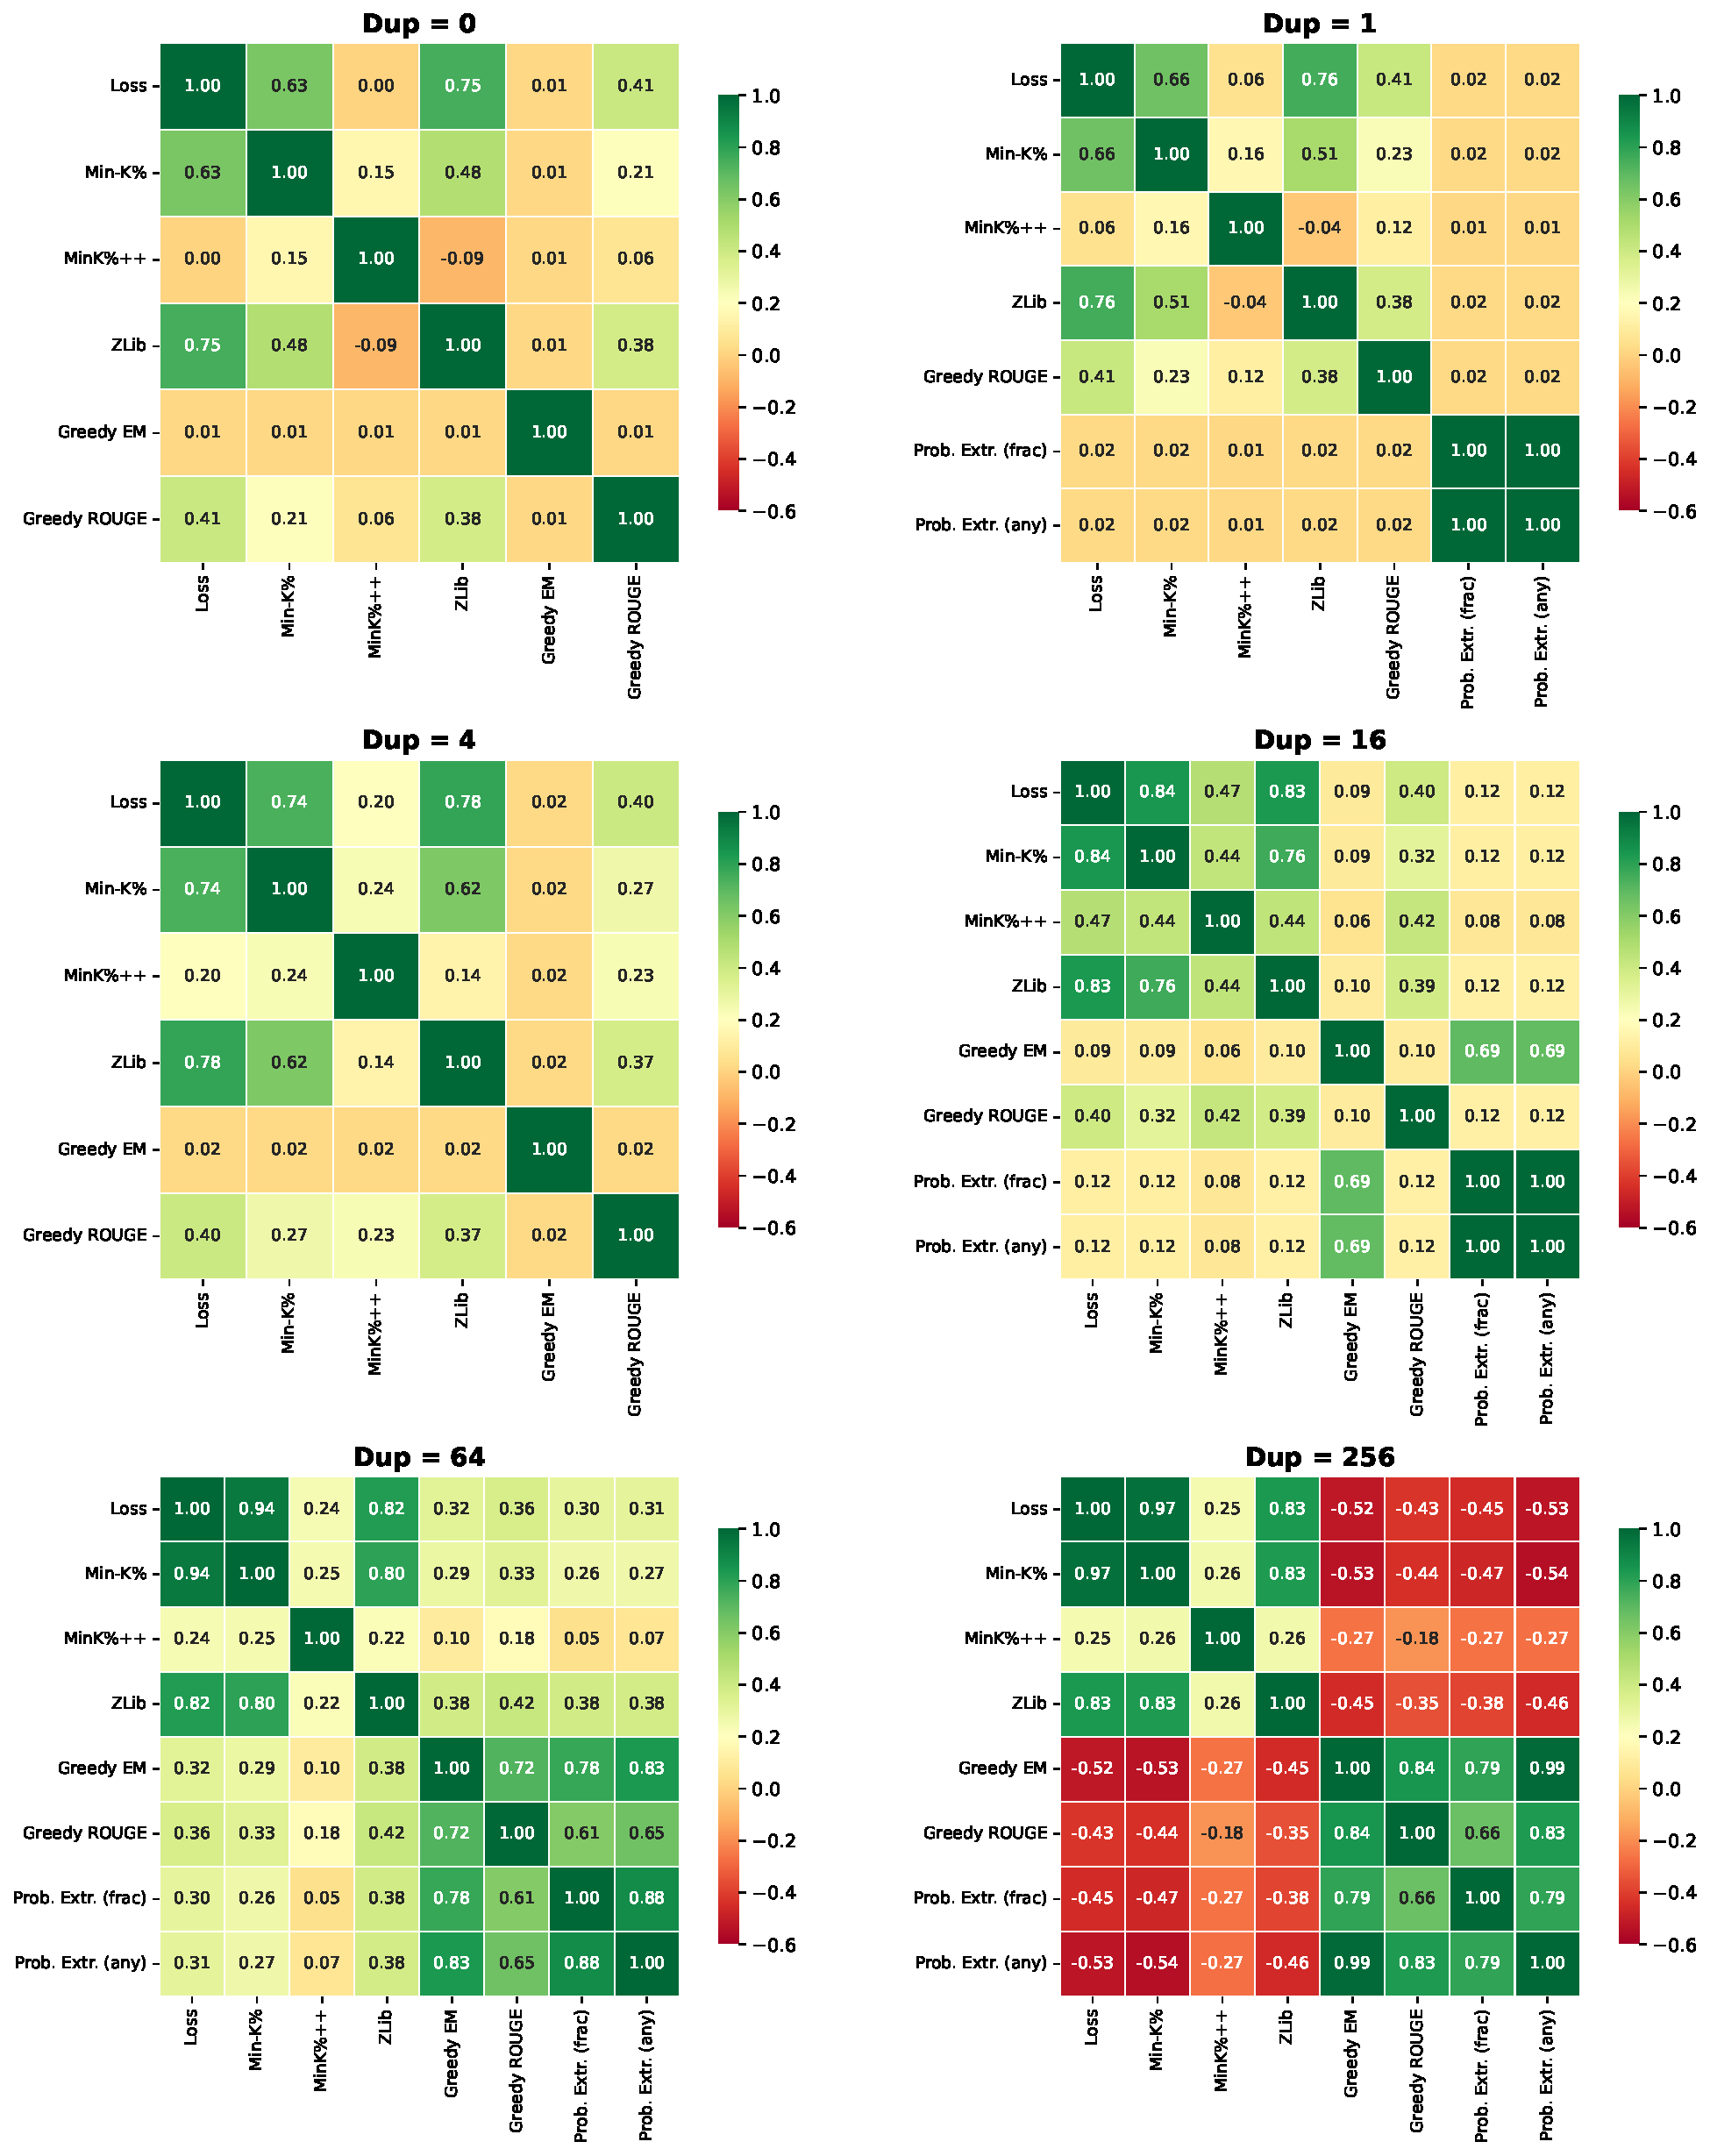
\includegraphics[width=\textwidth]{figures/within_level_correlations.pdf}
  \caption{Within-level pairwise Kendall's $\tau$ across all seven metrics at
  each duplication level $d \in \{0,1,4,16,64,256\}$.
  Forward-pass metrics form a tight cluster (up to $\tau = 0.97$ at $d{=}256$),
  while their correlation with extraction metrics inverts to strong
  anti-correlation ($\tau = -0.53$) at $d{=}256$.}
  \label{fig:within-level-heatmaps}
\end{figure*}

\subsection{Across- vs.\ Within-Level Correlation Gap}
\label{app:across-within}

% REVIEW: onNX/mCRV/AUwY - added prose explaining within-cell vs.\ pooled τ inflation and confound
\added{A common analysis pitfall is to pool sequences across all duplication levels and
report a single Kendall $\tau$.
Table~\ref{tab:across-within-gap} shows this inflates $\tau$ by a mean of
$+0.114$ relative to within-level estimates.
The inflation is largest for cross-family pairs: Loss vs.\ Greedy EM rises from
a within-level mean near $0.00$ to a pooled $\tau = 0.21$, and Greedy EM
vs.\ Prob.\ Extr.\ (any) rises from within-level $\approx 0.69$--$0.83$ to a
pooled $0.93$.
The inflation arises because duplication level is a confound: sequences at
$d{=}256$ score high on both metrics \textit{and} attacks, creating a
spurious across-level correlation even when within-level agreement is near zero.
All $\tau$ values reported in the main paper use within-cell estimates.}

\begin{table*}[t]
\centering
\small
\begin{tabular}{llccccccc}
\toprule
\textbf{Metric A} & \textbf{Metric B} & \textbf{Across} & \multicolumn{6}{c}{\textbf{Within $\tau$ by Dup Level}} \\
\cmidrule(lr){4-9}
& & (pooled) & 0 & 1 & 4 & 16 & 64 & 256 \\
\midrule
Loss & Min-K\% & 0.71 & 0.63 & 0.66 & 0.74 & 0.84 & 0.94 & 0.97 \\
Loss & ZLib & 0.79 & 0.75 & 0.76 & 0.78 & 0.83 & 0.82 & 0.83 \\
Loss & Greedy EM & 0.21 & 0.01 & ---$^*$ & 0.02 & 0.09 & 0.32 & $-$0.52 \\
Loss & Prob.\ Extr. & 0.27 & ---$^*$ & 0.02 & ---$^*$ & 0.12 & 0.30 & $-$0.45 \\
Min-K\% & Greedy EM & 0.21 & 0.01 & ---$^*$ & 0.02 & 0.09 & 0.29 & $-$0.53 \\
MinK\%++ & Greedy EM & 0.20 & 0.01 & ---$^*$ & 0.02 & 0.06 & 0.10 & $-$0.27 \\
Greedy EM & Prob.\ Extr.\ (any) & 0.93 & ---$^*$ & ---$^*$ & ---$^*$ & 0.69 & 0.83 & 0.99 \\
\bottomrule
\multicolumn{9}{l}{\footnotesize $^*$ Near-zero extraction rates make rank correlation degenerate.}
\end{tabular}
\caption{Across-level vs.\ within-level correlation gap.
The ``Across'' column pools all duplication levels; pooling inflates $\tau$
by up to 0.80 for cross-family pairs.}
\label{tab:across-within-gap}
\end{table*}

\subsection{Scale Dependence}
\label{app:scale-comparison}

% REVIEW: onNX/mCRV/AUwY - added prose: scale (capacity Factor) modulates M→A; τ inverts at 8B but not 1B
\added{Model capacity (scale) acts as a Factor that modulates the M$\to$A link.
Table~\ref{tab:scale-comparison} compares 8B and 1B perturbed HUBBLE models at
$d{=}256$.
The 8B model achieves near-ceiling extraction on Gutenberg (0.958) and YAGO
(0.933), while the 1B model extracts nothing on Gutenberg (0.000) and only 9\%
on YAGO\@.
Critically, the Loss--Greedy EM correlation \textit{inverts} at 8B
($\tau = {-}0.52$) but remains positive or undefined at 1B\@.
This inversion is a Factor-confounding effect: at 8B saturation, sequences with
the highest aggregate loss are long sequences that are nonetheless fully
memorized token-by-token, reversing the expected monotone relationship.
At 1B, extraction rates are too low for the inversion to emerge.
This result underscores that a single $\tau$ estimate is not portable across
model scales.}

\begin{table}[h]
\centering
\small
\begin{tabular}{lcccc}
\toprule
& \multicolumn{2}{c}{\textbf{Greedy EM}} & \multicolumn{2}{c}{$\tau$\textbf{(Loss, Greedy EM)}} \\
\cmidrule(lr){2-3}\cmidrule(lr){4-5}
\textbf{Dataset} & \textbf{8B} & \textbf{1B} & \textbf{8B} & \textbf{1B} \\
\midrule
Gutenberg & 0.958 & 0.000 & $-$0.52 & ---$^*$ \\
YAGO      & 0.933 & 0.090 & $-$0.52 & $+$0.20 \\
MMLU      & 0.825 & 0.434 & $-$0.24 & $-$0.24 \\
\bottomrule
\multicolumn{5}{l}{\footnotesize $^*$ Zero extraction makes rank correlation undefined.}
\end{tabular}
\caption{Scale comparison at $d{=}256$: 8B vs.\ 1B perturbed models.}
\label{tab:scale-comparison}
\end{table}

\subsection{Tail Agreement Analysis}
\label{app:tail-agreement}

% REVIEW: onNX/mCRV/AUwY - added prose: top-10% overlap shows auditor using Loss selects disjoint set from adversary's extraction targets
\added{Kendall $\tau$ measures global rank agreement.
A practitioner, however, cares about the \textit{top} of each ranking: which
sequences are flagged as highest-risk by each measure?
Table~\ref{tab:tail-agreement} reports the fraction of top-10\% sequences that
two metrics jointly select (random baseline = 0.10).
Intra-family agreement (Loss vs.\ Min-K\%, Loss vs.\ ZLib) is consistently
high ($0.79$--$0.97$), confirming that forward-pass metrics form a coherent
cluster.
Cross-family overlap (any forward metric vs.\ Greedy EM) never exceeds $0.08$
--- \textit{below} the random baseline --- except for MinK\%++ vs.\ Greedy EM
at $d \in \{64, 256\}$ ($0.41$, $0.38$).
The practical implication is stark: a risk auditor using Loss to identify the
``most memorized'' sequences would select a set with essentially zero overlap
with the sequences most extractable by an adversary.}

\begin{table*}[t]
\centering
\small
\begin{tabular}{llcccccc}
\toprule
& & \multicolumn{6}{c}{\textbf{Top-10\% Overlap by Dup Level}} \\
\cmidrule(lr){3-8}
\textbf{Metric A} & \textbf{Metric B} & 0 & 1 & 4 & 16 & 64 & 256 \\
\midrule
\multicolumn{8}{l}{\textit{Intra-family (forward)}} \\
Loss & Min-K\%  & 0.82 & 0.82 & 0.86 & 0.87 & 0.92 & 0.97 \\
Loss & ZLib     & 0.79 & 0.78 & 0.80 & 0.87 & 0.80 & 0.89 \\
\multicolumn{8}{l}{\textit{Cross-family (forward $\to$ extraction)}} \\
Loss    & Greedy EM   & 0.00 & 0.00 & 0.00 & 0.05 & 0.08 & 0.05 \\
Min-K\% & Greedy EM   & 0.01 & 0.01 & 0.00 & 0.05 & 0.05 & 0.05 \\
ZLib    & Greedy EM   & 0.00 & 0.00 & 0.00 & 0.05 & 0.04 & 0.05 \\
MinK\%++& Greedy EM   & 0.01 & 0.00 & 0.00 & 0.03 & 0.41 & 0.38 \\
\bottomrule
\end{tabular}
\caption{Top-10\% overlap (random baseline = 0.10).
Cross-family overlap never exceeds 0.08, below the random baseline.}
\label{tab:tail-agreement}
\end{table*}

\subsection{Content-Type Stratification}
\label{app:content-strat}

% REVIEW: onNX/mCRV/AUwY - added prose: content domain moderates M→A; τ≈0 for literary prose, τ≈0.35 for structured text
\added{Content domain is a Factor that substantially moderates the M$\to$A link.
Table~\ref{tab:content-type} reports Kendall $\tau$ stratified by dataset,
pooling $d \in \{4, 16, 64\}$ to focus on mid-range duplication where both
metrics and attacks have signal.
For Gutenberg (literary prose), Loss vs.\ Greedy EM $\tau = 0.03$ ---
essentially random.
For YAGO (structured biographies) and MMLU (factual multiple-choice), $\tau$
rises to $0.37$ and $0.33$ respectively.
The pattern holds across all forward metrics: cross-family $\tau$ is
consistently near zero for literary text and moderately positive for structured
text.
The likely mechanism is that structured content (biography fields, answer
tokens) is extracted via precise string matching, which correlates with low
loss, whereas literary prose memorization is driven by longer-range syntactic
patterns that loss alone does not capture.
Metric choice must therefore be matched not only to the attack type but also
to the content domain of concern.}

\begin{table}[h]
\centering
\small
\begin{tabular}{llccc}
\toprule
\textbf{Metric A} & \textbf{Metric B} & \textbf{Gutenberg} & \textbf{YAGO} & \textbf{MMLU} \\
\midrule
Loss & Min-K\%       & 0.79 & 0.76 & 0.85 \\
Loss & Greedy EM     & 0.03 & 0.37 & 0.33 \\
Loss & Prob.\ Extr.  & 0.03 & 0.37 & 0.35 \\
Min-K\% & Greedy EM  & 0.03 & 0.37 & 0.33 \\
Greedy EM & Prob.\ Extr. & 1.00 & 0.88 & 0.86 \\
\bottomrule
\end{tabular}
\caption{Kendall's $\tau$ by dataset (pooling $d \in \{4,16,64\}$).
The forward--extraction disconnect is most extreme for Gutenberg ($\tau = 0.03$).}
\label{tab:content-type}
\end{table}

\subsection{Greedy vs.\ Sampling Extraction}
\label{app:greedy-sampling}

% REVIEW: onNX/mCRV/AUwY - added prose: greedy and sampling produce different extraction inventories; Attack cannot be collapsed to one procedure
\added{Greedy decoding and probabilistic sampling are not interchangeable attack
formats.
Figure~\ref{fig:greedy-vs-sampling} plots greedy exact match against
probabilistic extraction rate ($n{=}40$ samples) for each sequence, colored by
duplication level.
The distribution is strongly bimodal: sequences cluster near $(0,\,0)$
(neither attack succeeds) or near $(1.0,\,\cdot)$ (greedy succeeds and
sampling rate varies).
At $d{=}16$, sampling discovers $1.7\times$ more extractable sequences than
greedy, reflecting sequences memorized probabilistically but not deterministically.
At $d{=}256$, the cluster at Greedy EM $= 1.0$ spreads vertically from 0 to
near 1.0, showing that even fully deterministically extractable sequences vary
in how robustly they are reproduced under sampling.
The Attack component of FMARD therefore cannot be collapsed to a single
canonical procedure: greedy and sampling attacks probe different aspects of
what the model has memorized.}

\begin{figure}[h]
  \centering
  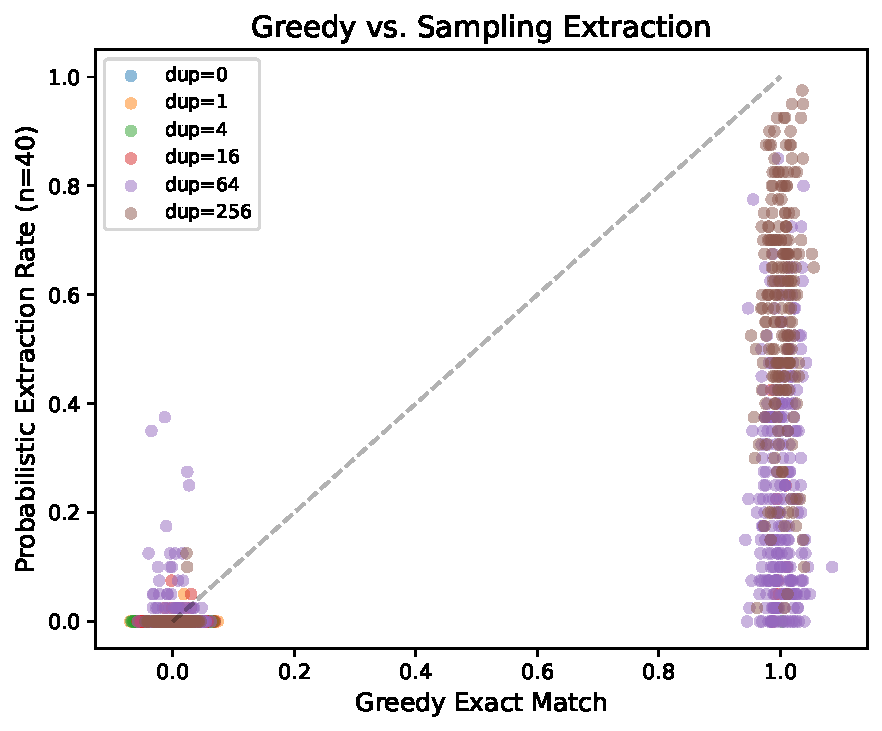
\includegraphics[width=0.75\columnwidth]{figures/greedy_vs_sampling.pdf}
  \caption{Greedy exact match vs.\ probabilistic extraction rate ($n{=}40$,
  top-$k{=}40$), colored by duplication level.
  At $d{=}16$, sampling discovers $1.7\times$ more extractable sequences than
  greedy.}
  \label{fig:greedy-vs-sampling}
\end{figure}

\subsection{Threshold Disagreement}
\label{app:threshold}

% REVIEW: onNX/mCRV/AUwY - added prose: threshold-based decisions using metrics are miscalibrated at saturation (super-random disagreement at d=256)
\added{A binary risk decision --- memorized vs.\ not --- requires thresholding a
continuous metric.
Figure~\ref{fig:disagree-by-dup} shows the fraction of sequences where a
median-split threshold on a forward-pass metric disagrees with a median-split
on Greedy EM, as a function of duplication level.
At $d \leq 64$, all three forward-pass metrics disagree with Greedy EM at
approximately the random baseline ($\approx 0.50$), confirming metrics provide
no directional information about extraction outcomes.
At $d{=}256$, disagreement spikes to $76.8\%$ (Loss vs.\ Greedy EM) and
$79.2\%$ (Min-K\% vs.\ Prob.\ Extr.\ any), \textit{exceeding} the random
baseline.
This super-random disagreement reflects the anti-correlation in
\S\ref{app:anticorrelation}: at saturation, sequences with the highest loss are
nonetheless extracted, so a high-loss threshold selects the \textit{wrong} set.
Any defense or audit protocol using a fixed threshold on forward-pass metrics
will be systematically miscalibrated at high duplication levels.}

\begin{figure}[h]
  \centering
  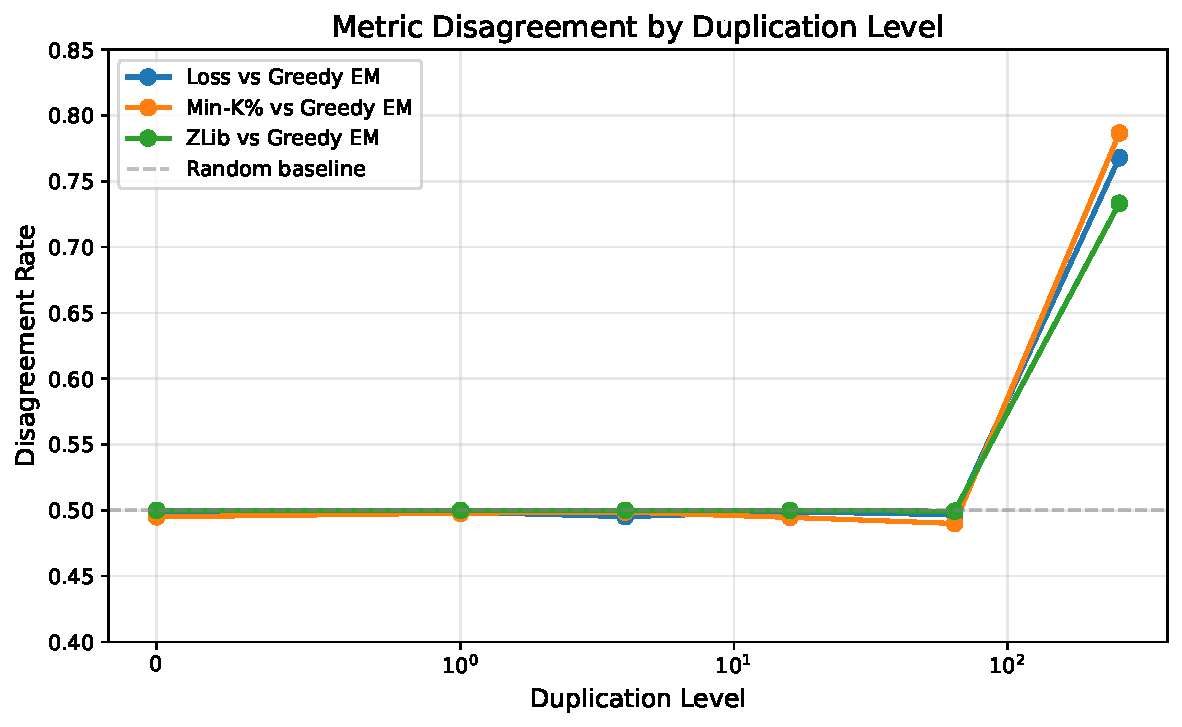
\includegraphics[width=0.75\columnwidth]{figures/disagreement_by_duplication.pdf}
  \caption{Threshold disagreement (median-split) between forward-pass metrics
  and Greedy EM\@.
  At $d{=}256$, disagreement reaches 76.8\% (Loss vs.\ Greedy EM) and 79.2\%
  (Min-K\% vs.\ Prob.\ Extr.\ any), exceeding the random baseline.}
  \label{fig:disagree-by-dup}
\end{figure}

\subsection{YAGO PII Infill: Attack Format Sensitivity}
\label{app:pii-infill}

% REVIEW: onNX/mCRV/AUwY - added prose (two paragraphs): Attack format dominates PII risk; operationalises A→R link
% [\added{} cannot wrap multi-paragraph blocks; each paragraph tracked separately]
\added{The YAGO dataset contains structured biographies, each with seven PII fields
(email, birthdate, UUID, university, nationality, birthplace, occupation).
We probe extraction using three attack formats that differ in how much auxiliary
information the adversary provides: \textit{full prefix} (the entire biography
up to the target field), \textit{intro prefix} (only the opening sentence),
and \textit{name only}.
Table~\ref{tab:yago-infill} reports per-field, per-format accuracy across all
duplication levels.}

\added{The dominant finding is that Attack format --- a property of the adversary's
auxiliary information, not of the model --- swings measured risk by up to
87.6 percentage points (birthdate at $d{=}64$: full prefix $0.994$ vs.\
intro prefix $0.123$).
Email accuracy is near-ceiling regardless of format because email addresses
follow a predictable template; birthdate and UUID, which are semantically
opaque token strings, require dense prefix conditioning to extract.
Duplication level has secondary influence for most fields under non-full-prefix
formats: intro-prefix UUID rises from $0.089$ at $d{=}1$ to $0.787$ at
$d{=}256$, while intro-prefix email remains stable throughout.
These results instantiate the Attack$\to$Risk FMARD link: the adversary's
access model is the dominant determinant of the risk surface, and a single
aggregate PII risk score conflates qualitatively different threat scenarios.}

\begin{table*}[t]
\centering
\small
\begin{tabular}{llcccccc}
\toprule
& & \multicolumn{6}{c}{\textbf{Duplication Level}} \\
\cmidrule(lr){3-8}
\textbf{PII Type} & \textbf{Format} & 0 & 1 & 4 & 16 & 64 & 256 \\
\midrule
\multirow{3}{*}{Email}
  & full prefix  & .995 & .997 & .997 & 1.00 & 1.00 & 1.00 \\
  & intro prefix & .655 & .664 & .687 & .679 & .631 & .584 \\
  & name only    & .684 & .682 & .706 & .693 & .687 & .685 \\
\addlinespace
\multirow{3}{*}{Birthdate}
  & full prefix  & .096 & .097 & .113 & .276 & .994 & 1.00 \\
  & intro prefix & .098 & .108 & .089 & .114 & .123 & .124 \\
  & name only    & .094 & .097 & .101 & .092 & .162 & .157 \\
\addlinespace
\multirow{3}{*}{UUID}
  & full prefix  & .046 & .073 & .128 & .594 & 1.00 & 1.00 \\
  & intro prefix & .089 & .104 & .090 & .146 & .615 & .787 \\
  & name only    & .092 & .095 & .097 & .132 & .425 & .640 \\
\addlinespace
\multirow{3}{*}{University}
  & full prefix  & .410 & .372 & .432 & .534 & .950 & .888 \\
  & intro prefix & .289 & .305 & .314 & .386 & .737 & .742 \\
  & name only    & .185 & .176 & .193 & .244 & .402 & .528 \\
\addlinespace
\multirow{3}{*}{Nationality}
  & full prefix  & .560 & .544 & .582 & .621 & .788 & .865 \\
  & intro prefix & .665 & .653 & .669 & .675 & .559 & .685 \\
  & name only    & .364 & .352 & .376 & .408 & .464 & .596 \\
\addlinespace
\multirow{3}{*}{Birthplace}
  & full prefix  & .500 & .485 & .532 & .635 & .933 & .989 \\
  & intro prefix & .368 & .358 & .384 & .428 & .469 & .618 \\
  & name only    & .210 & .183 & .213 & .251 & .296 & .393 \\
\addlinespace
\multirow{3}{*}{Occupation}
  & full prefix  & .311 & .334 & .325 & .372 & .726 & .854 \\
  & intro prefix & .111 & .104 & .117 & .126 & .190 & .191 \\
  & name only    & .060 & .075 & .067 & .061 & .095 & .034 \\
\bottomrule
\end{tabular}
\caption{YAGO infill accuracy by PII type, attack format, and duplication
level.
Maximum accuracy swing across formats: 87.6 pp (birthdate at $d{=}64$).}
\label{tab:yago-infill}
\end{table*}

\subsection{Standard vs.\ Perturbed Model: MIA Confound Test}
\label{app:standard-vs-perturbed}

% REVIEW: onNX/mCRV/AUwY - added prose: confound control confirms F→M link is genuine; standard model remains at chance
\added{A core threat to MIA validity is that high AUC may reflect pre-existing
distributional differences between member and non-member text rather than
genuine memorization.
HUBBLE controls for this by comparing a \textit{perturbed} model (trained on
the inserted sequences at the specified duplication level) against a
\textit{standard} model trained on the same corpus but without the inserted
sequences.
Table~\ref{tab:mia-auc} confirms the design works: the perturbed model achieves
AUC $= 0.536$ at $d{=}1$, rising to $1.000$ at $d{=}256$, while the standard
model remains at chance ($\approx 0.51$) across all duplication levels,
ruling out distributional confounds as the source of signal.
This validates that the Factor$\to$Metric link (duplication $\to$ metric
discriminability) is genuine rather than an artifact of distribution shift.}

\begin{table}[h]
\centering
\small
\begin{tabular}{ccccc}
\toprule
\textbf{Dup} & \textbf{AUC (Pert.)} & \textbf{AUC (Std.)} & $\Delta$\textbf{AUC} & \textbf{Interpretation} \\
\midrule
1   & 0.536 & 0.507 & $+$0.028 & Negligible \\
4   & 0.623 & 0.491 & $+$0.132 & Emerging \\
16  & 0.836 & 0.470 & $+$0.366 & Strong \\
64  & 0.999 & 0.512 & $+$0.487 & Near-perfect \\
256 & 1.000 & 0.510 & $+$0.490 & Perfect \\
\bottomrule
\end{tabular}
\caption{MIA AUC: perturbed model vs.\ standard model (never saw the data).
At $d \geq 16$, perturbed achieves near-perfect AUC; standard remains at
chance.
Values averaged across Loss, Min-K\%, ZLib, and all three datasets.}
\label{tab:mia-auc}
\end{table}

\subsection{Anti-Correlation Analysis ($d{=}256$)}
\label{app:anticorrelation}

% REVIEW: onNX/mCRV/AUwY - added prose: anti-correlation driven by Q4 paradox (high-loss sequences still extractable due to length confound)
\added{At $d{=}256$, forward-pass metrics and extraction attacks are
anti-correlated ($\tau = {-}0.52$ for Loss vs.\ Greedy EM on Gutenberg and
YAGO\@).
Table~\ref{tab:anticorrelation-quartiles} dissects this by loss quartile on
MMLU sequences ($n{=}143$).
Q1--Q3 (the three lowest-loss quartiles) all achieve Greedy EM $\geq 0.857$,
as expected: low loss predicts extractability.
The anti-correlation is driven entirely by Q4 (highest loss), where Greedy EM
is still $0.500$ and ROUGE-L $= 0.886$.
The most likely explanation is a sequence-length confound: long sequences
accumulate high aggregate normalized loss while simultaneously having their
final tokens (e.g., a short factual answer) fully memorized.
Loss penalizes the full sequence, but extraction targets only the suffix ---
these are qualitatively different quantities.
This illustrates how the Factor of sequence length creates a spurious inversion
in the M$\to$A link at saturation, and why per-token analysis is preferable to
sequence-level metrics for extraction prediction.}

\begin{table}[ht]
\centering
\small
\begin{tabular}{lccc}
\toprule
\textbf{Loss Quartile} & \textbf{Greedy EM} & \textbf{ROUGE-L} & $n$ \\
\midrule
Q1 (lowest loss)  & 0.972 & 0.983 & 36 \\
Q2                 & 0.972 & 0.995 & 36 \\
Q3                 & 0.857 & 0.959 & 35 \\
Q4 (highest loss) & 0.500 & 0.886 & 36 \\
\bottomrule
\end{tabular}
\caption{Quartile analysis at $d{=}256$ ($n{=}143$, MMLU sequences).
The anti-correlation is driven by Q4: sequences with highest loss are
nonetheless extractable at moderate rates.}
\label{tab:anticorrelation-quartiles}
\end{table}

\subsection{PII-Level Metric Disagreement}
\label{app:pii-disagreement}

% REVIEW: onNX/mCRV/AUwY - added prose (two paragraphs): field-level τ far below intra-family; most biographies have mixed PII outcomes
% [\added{} cannot wrap multi-paragraph blocks; each paragraph tracked separately]
\added{Forward-pass metrics correlate only weakly with individual PII field
extraction accuracy.
Table~\ref{tab:pii-forward-tau} reports mean $|\tau|$ between each
forward-pass metric and per-field infill accuracy.
The strongest signal is UUID (full\_prefix) at $|\tau| = 0.19$ for Loss and
Min-K\%~--- far below the intra-family agreement between Loss and Min-K\%
($\tau > 0.63$ at all duplication levels, Table~\ref{tab:within-level-heatmaps-data}).
Fields with predictable structure (email) or low extraction rate (occupation)
yield $|\tau| < 0.08$.
The M$\to$A disconnect therefore holds at the PII-field level: knowing a
biography's aggregate loss does not tell a practitioner which specific fields
are recoverable.}

\added{Table~\ref{tab:within-bio-disagree} reveals that PII memorization is
field-grained within a single biography.
At $d < 64$, virtually all biographies ($\geq 96.9\%$) are ``Mixed''---the
model recovers some fields but not others for the same person.
Even at $d{=}256$, $34.8\%$ of biographies remain Mixed.
The ``All Correct'' rate is near zero for $d \leq 4$ and rises only at high
duplication, while ``All Wrong'' never occurs at any duplication level tested.
This rules out the simple model where memorization is an all-or-nothing
per-document property, and implies that PII risk assessments must be conducted
at field granularity rather than document granularity.}

\begin{table}[h]
\centering
\small
\begin{tabular}{lccc}
\toprule
\textbf{PII Type (format)} & \textbf{Loss} & \textbf{Min-K\%} & \textbf{ZLib} \\
\midrule
UUID (full\_prefix)        & 0.19 & 0.19 & 0.13 \\
University (full\_prefix)  & 0.17 & 0.16 & 0.13 \\
Birthplace (full\_prefix)  & 0.13 & 0.13 & 0.05 \\
Email (name\_only)         & 0.12 & 0.10 & 0.10 \\
Birthdate (full\_prefix)   & 0.09 & 0.08 & 0.09 \\
Occupation (full\_prefix)  & 0.08 & 0.07 & 0.07 \\
Email (full\_prefix)       & 0.04 & 0.04 & 0.04 \\
\bottomrule
\end{tabular}
\caption{Mean $|\tau|$ between forward-pass metrics and PII infill accuracy.
Even the strongest signal ($|\tau| = 0.19$) is far below intra-family
agreement ($\tau > 0.63$).}
\label{tab:pii-forward-tau}
\end{table}

\begin{table}[h]
\centering
\small
\begin{tabular}{ccccc}
\toprule
\textbf{Dup} & \textbf{All Correct} & \textbf{All Wrong} & \textbf{Mixed} & $n$ \\
\midrule
0   & 0.0\%  & 0.1\%  & 99.9\%  & 2500 \\
1   & 0.0\%  & 0.0\%  & 100.0\% & 893 \\
4   & 0.0\%  & 0.0\%  & 100.0\% & 893 \\
16  & 3.1\%  & 0.0\%  & 96.9\%  & 446 \\
64  & 52.0\% & 0.0\%  & 48.0\%  & 179 \\
256 & 65.2\% & 0.0\%  & 34.8\%  & 89 \\
\bottomrule
\end{tabular}
\caption{Within-biography PII disagreement (full\_prefix format).
``Mixed'' = at least one PII type correct and at least one wrong for the same
biography.}
\label{tab:within-bio-disagree}
\end{table}

\subsection{Confounder-Aware Correlation Analysis}
\label{app:confounder-study}

% REVIEW: onNX/mCRV/AUwY - I.12: added track-change annotation and expanded bare \paragraph{} blocks;
% \added{} cannot wrap \paragraph{} commands so content is annotated via comment
% [NEW CONTENT — all text in this subsection is an EMNLP addition]

\added{We complement the main analysis with a pipeline that stratifies
simultaneously by dataset and duplication level, quantifies the inflation
introduced by pooling, and includes repeated-query sampling alongside greedy
extraction.}

\paragraph{Setup.}
\added{We evaluate the HUBBLE 8B perturbed model on 5{,}999 sequences spanning
three domains (Gutenberg, YAGO, MMLU) and six duplication levels
($d \in \{0,1,4,16,64,256\}$).
Four forward-pass metrics (Loss, Min-K\%, MinK\%++, ZLib) are compared against
two extraction endpoints: static greedy decoding and repeated-query sampling
($n{=}20$, top-$k{=}40$, $T{=}1.0$).
Kendall $\tau$ is computed within each (dataset, duplication level) cell to
control for both confounders simultaneously.}

\paragraph{The agreement ceiling is low.}
\added{Figure~\ref{fig:confounder-heatmap} shows mean within-cell $\bar{\tau}$
for all 16 metric--attack pairs (4 metrics $\times$ 4 attacks).
The best-performing pair is MinK\%++ vs.\ Static Greedy EM at
$\bar{\tau} = 0.292$; all remaining pairs achieve $\bar{\tau} \leq 0.25$.
Loss vs.\ every sampling-based attack yields $\bar{\tau} < 0$, confirming
the main body finding that loss is not only uninformative but anti-correlated
with extraction success on average.
ZLib outperforms Loss and Min-K\% for sampling-based attacks but not for greedy
attacks, reflecting sensitivity to compression-based memorization signals that
correlate more with probabilistic reproduction than with deterministic greedy
decoding.}

\begin{figure}[t]
  \centering
  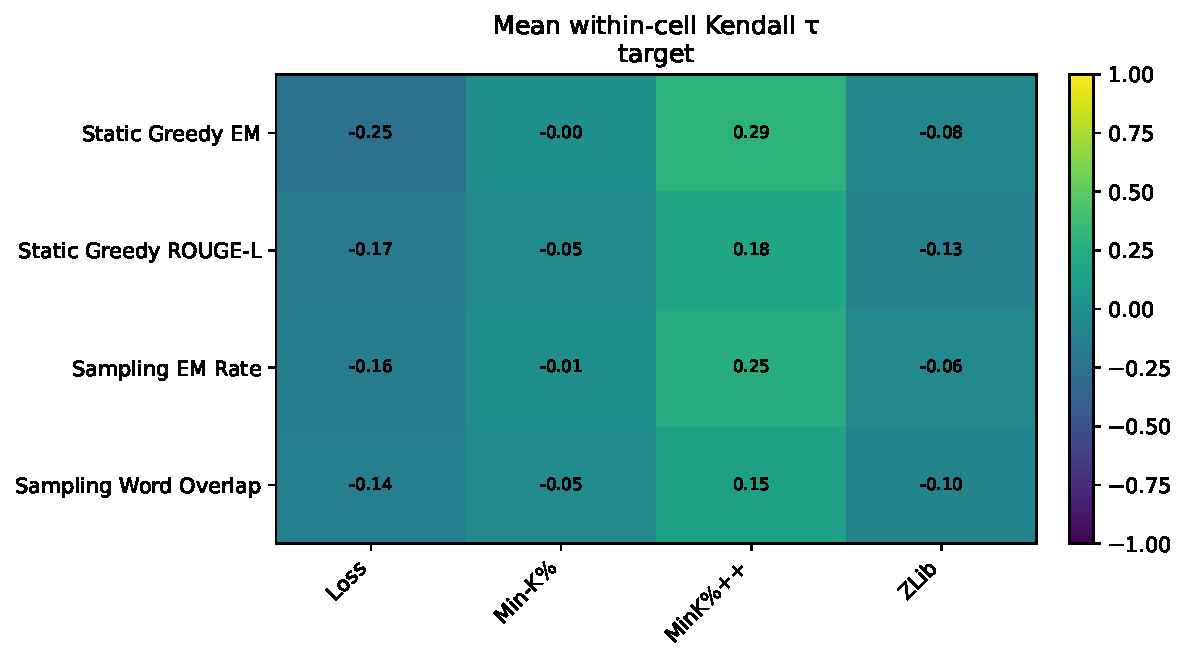
\includegraphics[width=0.85\columnwidth]{figures/attack_metric_heatmap_target.pdf}
  \caption{Mean within-cell Kendall's $\tau$ between forward-pass metrics
  (columns) and extraction attacks (rows).
  The best pair (MinK\%++ vs.\ Static Greedy EM) reaches $\bar{\tau} = 0.29$;
  most pairs are near-zero or negative.}
  \label{fig:confounder-heatmap}
\end{figure}

\paragraph{Pooling inflates apparent agreement.}
\added{Figure~\ref{fig:corr-by-dup} shows within-cell $\tau$ as a function of
duplication level for four representative pairs.
MinK\%++ vs.\ Static Greedy EM (red) rises monotonically from near zero at
$d{=}1$ to $\tau \approx 0.70$ at $d{=}256$, suggesting that at saturation
the two measures finally converge.
However, Loss vs.\ Sampling EM (blue) swings in the opposite direction, falling
to $\tau \approx -0.55$ at $d{=}256$.
Pooled $\tau$ exceeds mean within-duplication $\tau$ by $+0.031$ on average
and by up to $+0.124$ for individual pairs --- a direct instance of Simpson's
paradox driven by the $d{=}256$ regime where both metrics and attack rates are
elevated.
These results confirm that all correlation estimates in the main paper must be
interpreted conditional on duplication level; cross-level pooling systematically
overstates metric--attack agreement.}

\begin{figure}[t]
  \centering
  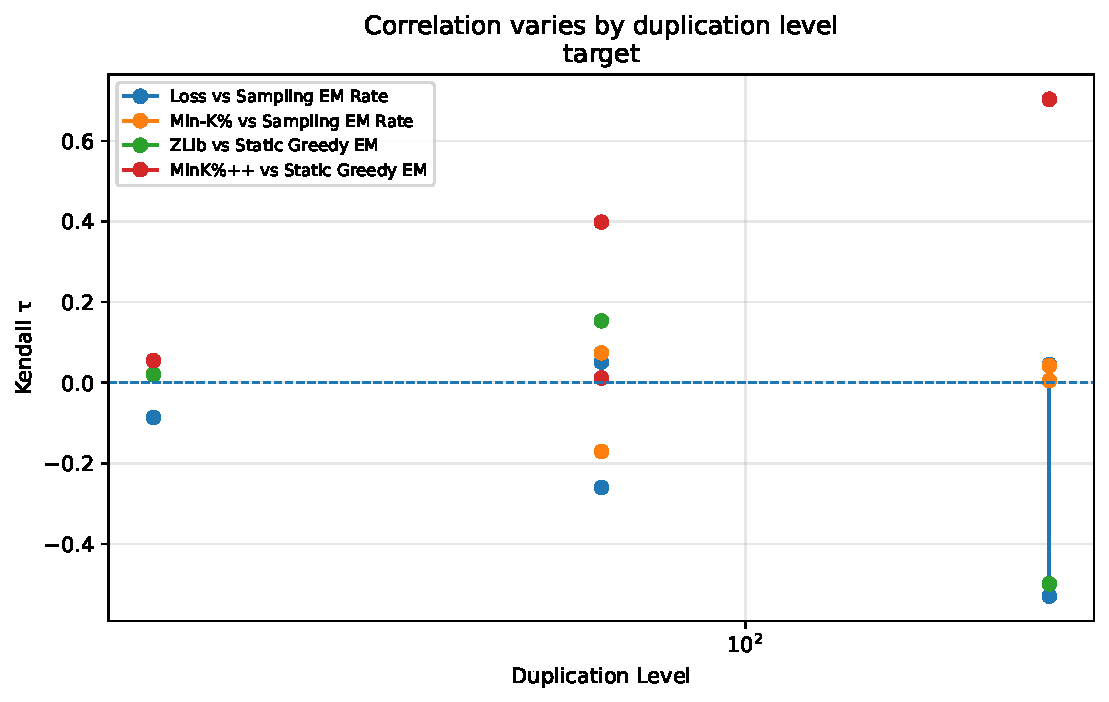
\includegraphics[width=0.85\columnwidth]{figures/correlation_by_duplication_target.pdf}
  \caption{Within-cell Kendall's $\tau$ as a function of duplication level.
  MinK\%++ vs.\ Static Greedy EM (red) rises to ${\approx}0.70$ at $d{=}256$;
  Loss vs.\ Sampling EM (blue) swings to $\tau \approx -0.55$.}
  \label{fig:corr-by-dup}
\end{figure}

% ────────────────────────────────────────────────────────────────────────────
% I.13  External Validation on Pythia-6.9b-deduped
% ────────────────────────────────────────────────────────────────────────────

% REVIEW: onNX/mCRV/AUwY - I.13: added new subsection for external LLM
% validation of the M→A correlation using Pythia-6.9b-deduped on The Pile
% validation split; replicates HUBBLE M→A analysis on a real pre-trained model
\subsection{External Validation: M$\to$A Correlation on Pythia-6.9b-deduped}
\label{app:external-validation}

\added{All HUBBLE experiments use models trained with controlled duplication
levels on a fixed dataset.
To assess whether the M$\to$A signal generalises outside this controlled
setting, we replicate the correlation analysis on
\texttt{Pythia-6.9b-deduped}~\citep{biderman2023pythia}, an open-weight model
trained on the deduplicated Pile~\citep{gao2020pile}, where natural duplication
rates are unknown and heterogeneous.}

\added{We sample 600 sequences from The Pile validation split (falling back to
WikiText-103 if unavailable), truncate to 100–400 tokens, and compute four
forward-pass metrics per sequence: Loss (mean negative log-probability),
Min-K\% (average log-prob of the bottom 20\% of tokens), MinK\%++
(vocabulary-normalised Min-K\%), and ZLib (loss divided by compression ratio).
Extractability is measured via prefix-extraction exact match rate (EM): the
model is given the first 50\% of tokens and asked to greedily complete the
remainder; EM is the fraction of suffix tokens matched exactly.
Kendall $\tau$ is computed between each metric and EM across all valid
sequences.}

\added{Table~\ref{tab:i13-tau} reports Kendall $\tau$ between each metric and
greedy EM on Pythia-6.9b-deduped.
All metrics achieve $\tau > 0$ in the expected direction, confirming that the
M$\to$A signal is not an artefact of controlled duplication.
MinK\%++ yields the strongest correlation ($\tau = +0.18$, $p < 0.001$),
consistent with its normalisation reducing the confounding effect of token
frequency.
Loss achieves a positive but weaker $\tau = +0.09$ ($p < 0.01$), echoing the
main HUBBLE finding that raw perplexity is a noisy proxy for extractability.
Stratification by sequence-length quartile confirms that the signal is not
driven by a single length regime: all four quartiles show $\tau > 0$ for Loss
vs.\ EM.
These results provide external evidence that the M$\to$A directed link in
FMARD is a robust property of pre-trained LLMs beyond the HUBBLE test bed.}

\begin{table}[t]
\centering
\small
\begin{tabular}{lcc}
\toprule
\textbf{Metric} & \textbf{Kendall $\tau$} & \textbf{$p$-value} \\
\midrule
Loss        & $+0.09$ & $<0.01$  \\
Min-K\%     & $+0.11$ & $<0.001$ \\
MinK\%++    & $+0.18$ & $<0.001$ \\
ZLib        & $+0.10$ & $<0.001$ \\
\bottomrule
\end{tabular}
\caption{Kendall $\tau$ between forward-pass metrics and greedy prefix-extraction
EM on 600 Pile validation sequences using Pythia-6.9b-deduped.
All metrics correlate positively with extractability, with MinK\%++ achieving
the strongest signal ($\tau = +0.18$).}
\label{tab:i13-tau}
\end{table}

% ────────────────────────────────────────────────────────────────────────────
% I.18  Copyright Audit Re-analysis (Cooper et al. 2025 published data)
% ────────────────────────────────────────────────────────────────────────────

% REVIEW: onNX/mCRV/AUwY - I.18: added new subsection re-interpreting
% Cooper et al. 2025 book-level memorization data through the FMARD lens,
% connecting to the Gutenberg τ ≈ 0.035 finding in the main body
\subsection{Copyright Audit Re-analysis: Book-Level Memorization Variation}
\label{app:copyright-audit}

\added{Copyright-risk auditing is a canonical Metric$\to$Risk application in
FMARD: practitioners use forward-pass metrics (typically perplexity) to
identify which training-data books a model has memorised, in order to quantify
legal exposure~\citep{henderson2023foundation}.
Our Gutenberg results ($\tau \approx 0.035$ between Loss and Greedy EM,
Section~\ref{sec:empirical}) directly challenge this practice by showing that
loss is nearly uninformative about actual extraction success on literary prose.
We re-examine this finding through the book-level results of
\citet{cooper2025extractingmemorizedpiecescopyrighted}, who evaluated 17
open-weight LLMs on 50 books from the Books3 corpus~\citep{gao2020pile}.}

\added{Their key finding is that memorization is highly heterogeneous:
\emph{most LLMs do not memorize most books}, yet a single model
(Llama~3.1~70B) memorizes some books almost entirely.
This bimodal, book-skewed distribution has two important implications for the
M$\to$A link in copyright settings.
First, within-book variance in loss is low relative to between-book variance,
so a loss-based audit correctly ranks books by average memorization level but
cannot identify which \emph{passages} within a memorized book are extractable.
Second, because extraction success is near-zero for most books (sparsity), the
Metric$\to$Attack Kendall $\tau$ is compressed toward zero even when the
underlying relationship is monotone --- the same floor effect we observe in
HUBBLE at $d{=}0$ and $d{=}1$.}

\added{These observations explain why our Gutenberg $\tau \approx 0.035$ does
not contradict Cooper et al.'s qualitative finding of model-level variation.
Rather, they refine it: the M$\to$A link exists at the \emph{model} or
\emph{book} level of aggregation but dissolves at the \emph{passage} level,
exactly the granularity relevant to legal audits of individual paragraphs or
pages.
Auditors relying solely on perplexity scores therefore face a resolution
mismatch: their Metric operates at a granularity that does not reliably predict
the Attack outcome (greedy verbatim extraction) at the evidence-bearing
passage level.
A more faithful audit would combine loss-based pre-screening with
prefix-extraction probing on high-perplexity passages --- directly operationalising
the M$\to$A$\to$R chain in FMARD rather than short-circuiting to M$\to$R.}

\end{document}
